\documentclass[aps,prl,twocolumn,superscriptaddress,amsmath,amssymb,floatfix]{revtex4-2}
\usepackage{graphicx}
\usepackage{xcolor}
\usepackage[colorlinks=true,allcolors=blue]{hyperref}
\newcommand{\TODO}[1]{\textcolor{red}{[#1]}}
\begin{document}
\title{Zero-point flux fluctuations switch a quantum-dot Josephson loop from $0$ to $\pi$}
% Authors to be added.
\begin{abstract}
A superconducting loop closed by a quantum-dot Josephson junction and sharing its inductance with
a microwave mode is a $\pi$ loop whenever the dot is in its doublet state. We solve the full
electron--photon problem of this circuit, an interacting Anderson impurity in a BCS ring threaded by
the quantized flux of a lumped $LC$ mode, by DMRG, with the Peierls vertex $e^{ig(a+a^\dagger)}$ kept to all
orders. Three results follow. (i) The zero-point flux of the mode moves the singlet--doublet ($0$--$\pi$)
boundary of the junction: at a mode impedance $Z\simeq2\,{\rm k}\Omega$ ($g\simeq0.5$) a junction that is a $0$ junction
in isolation becomes a $\pi$ junction, by an amount that crosses over from the adiabatic flux average at
$\hbar\omega\ll E_A$ to the Franck--Condon reduction $t_J\to t_Je^{-g^2/2}$ of the tunnelling when $\hbar\omega$
exceeds the Andreev scale. (ii) Deep in the adiabatic regime the exact solution reduces, to $10^{-5}\Delta$ in
energy and $0.2\%$ in current, to an rf-SQUID (fluxonium) Hamiltonian with the microscopic $E(\varphi)$ of the
junction: the ``photon condensate'' with $\langle a\rangle\neq0$ is the classical screening instability
$\beta=2\pi LI_c/\Phi_0>1$, its ground state is the cat state of the two persistent-current directions, and
the threshold is pushed above $\beta=1$ by the zero-point motion of the flux. (iii) The electron$\times$photon
product state used in recent mean-field treatments of this circuit orders where the exact solution does not,
both for $E_J\lesssim3\hbar\omega$ and at the $0$--$\pi$ boundary, where a static moment replaces the Kramers
doublet. We give the parameters, in Al and NbTiN, at which the flux-driven parity switch and the cat state
are observable in two-tone spectroscopy.
\end{abstract}
\maketitle
% ------------------------------------------------------------------
%  Main body (PRL format) -- no title/abstract/intro/conclusion yet.
%  Compile with paper/main.tex (revtex4-2).
% ------------------------------------------------------------------

\begin{figure}[t]
  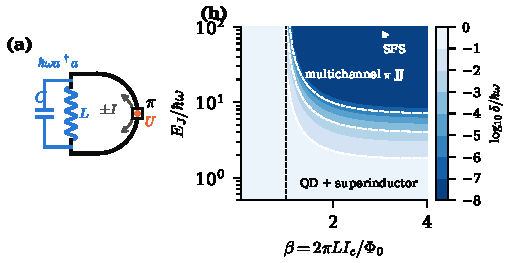
\includegraphics[width=\columnwidth]{../figs/fig_overview.pdf}
  \caption{\label{fig:overview}%
  (a) A superconducting loop closed by a $\pi$ junction (here an interacting dot
  with charging energy $U$) shares its inductance $L$ with an LC mode; the two
  degenerate states carry opposite persistent currents $\pm I$.
  (b) Tunnel splitting $\delta$ between the two current-carrying states in the
  plane of the screening parameter $\beta$ and the quantum parameter $E_J/\hbar\omega$
  [Eq.~\eqref{eq:BO} with the DMRG $E(\varphi)$ of the $U=2t$ junction]. White
  lines: $\delta/\hbar\omega=10^{-6},10^{-3},10^{-1}$; dashed: classical threshold $\beta=1$.
  Labels: typical regimes of the platforms discussed in the text.}
\end{figure}

\paragraph*{Model.}
We consider a superconducting (SC) loop of $L$ sites closed by an interacting
quantum dot (site $0$) and threaded by the magnetic flux of a single lumped LC mode
[Fig.~\ref{fig:overview}(a)]. The full microscopic Hamiltonian is
\begin{align}
  H &= \hbar\omega\, a^\dagger a
     -t\sum_{r=1}^{L-2}\sum_\sigma\left(c^\dagger_{r+1\sigma}c_{r\sigma}+{\rm h.c.}\right)
     +\Delta\sum_{r=1}^{L-1}\left(c^\dagger_{r\uparrow}c^\dagger_{r\downarrow}+{\rm h.c.}\right)
     \nonumber\\
    &\quad +\epsilon_d\, n_0 + U n_{0\uparrow}n_{0\downarrow}
     -t_J\sum_\sigma\left(c^\dagger_{0\sigma}c_{L-1\,\sigma}+{\rm h.c.}\right)
     \nonumber\\
    &\quad -t_J\sum_\sigma\left(e^{i\varphi_{\rm cl}}\,e^{ig(a+a^\dagger)}\,c^\dagger_{1\sigma}c_{0\sigma}+{\rm h.c.}\right).
  \label{eq:H}
\end{align}
The first line is the resonator and an $s$-wave BCS chain (hopping $t$, pairing $\Delta$);
the second line is the Anderson impurity (level $\epsilon_d=-U/2$, on-site
repulsion $U$) tunnel-coupled ($t_J$) to the two ends of the chain; the third line
carries the total Peierls phase of the loop, which by a gauge choice is placed on a
single bond. The vector potential of the mode enters through the gauge-invariant
displacement operator $D=e^{ig(a+a^\dagger)}$, so diamagnetic ($A^2$) terms are
included to all orders; $g=2\pi\Phi_{\rm zpf}/(h/e)$ is the electron phase generated
by the zero-point flux of the mode, and $\varphi_{\rm cl}$ is a static external
flux. An electron phase $\varphi=\pi$ corresponds to one superconducting flux
quantum $\Phi_0=h/2e$. For a lumped resonator of impedance $Z$, galvanically sharing
its inductance with the loop, $(2g)^2=\pi Z/R_Q$ with $R_Q=h/4e^2$. Unless stated
otherwise we take $t=1$, $\Delta=t$, $t_J=0.5t$, $L=14$ ($L\gg\xi$), $\hbar\omega=7.6\times10^{-4}t$
and \emph{no} external flux, $\varphi_{\rm cl}\to0^+$ (a seed $\varphi_{\rm cl}=10^{-3}$ is
used to select one of the degenerate states). Two auxiliary versions are also
used: a weak link ($U=0$, dot replaced by a bond $t_J$) biased by $\Phi_0/2$, and the
short ring with a Zeeman-polarized dot of Ref.~\cite{notebook}.
We write Eq.~\eqref{eq:H} compactly as
$H=\hbar\omega a^\dagger a+H_{\rm ring}[\varphi_{\rm cl}+g(a+a^\dagger)]$.

The only property of $H_{\rm ring}$ that enters below is its ground-state
energy at fixed phase,
\begin{equation}
  E(\varphi)=\sum_{m\ge 0}E_m\cos m\varphi .
  \label{eq:harm}
\end{equation}
Even harmonics ($m=2,4,\dots$) describe Cooper-pair tunnelling ($h/2e$
periodicity). The $m=1$ term is the single-electron ($h/e$) persistent
current of a mesoscopic ring~\cite{LossGoldbart1991} and is suppressed as $e^{-L/\xi}$. A
$0$-junction has $E_2<0$ and a $\pi$-junction has $E_2>0$. When a $0$-junction
is biased by $\Phi_0/2$, $\varphi_{\rm cl}=\pi/2$ maps $E_2\cos2\varphi\to-E_2\cos2\varphi$.
The two routes to a $\pi$ loop are therefore equivalent up to the odd harmonics,
which turn into an explicit symmetry-breaking term
$-E_1\sin\varphi$. In contrast, an intrinsic $\pi$-junction keeps
$E(\varphi)=E(-\varphi)$ exactly, since $H_{\rm ring}[0]$ is real
(time-reversal symmetry).

\paragraph*{Adiabatic reduction and Landau theory.}
For $\hbar\omega$ well below the Andreev gap $E_A$, the electrons follow the
flux adiabatically. To leading order in $\hbar\omega/E_A$, Eq.~\eqref{eq:H}
reduces to a single-particle problem for the dimensionless flux $X=a+a^\dagger$,
\begin{equation}
  H_{\rm BO}=\frac{\hbar\omega}{4}\left(P^2+X^2\right)+E(\varphi_{\rm cl}+gX),
  \qquad [X,P]=2i .
  \label{eq:BO}
\end{equation}
Equation~\eqref{eq:BO} is the Hamiltonian of an rf-SQUID~\cite{Friedman2000} whose inductive energy
is supplied by the mode. Writing it in the Cooper-pair phase
$\theta=2gX$ gives $4E_C n^2+\tfrac12E_L\theta^2+E(\theta/2)$ with
$E_L=\hbar\omega/8g^2$ and $E_C=\hbar\omega g^2$. A static field ($\langle a\rangle\neq0$),
i.e.\ a photon condensate carrying a persistent current
$I=-(2e/\hbar)\partial_\varphi E$, appears classically when the orbital response of the
ring at the symmetric point is paramagnetic and exceeds the stiffness of the mode,
\begin{equation}
  \beta\equiv\frac{2g^2\,|E''(\varphi_0)|}{\hbar\omega}>1,
  \qquad E''(\varphi_0)<0 .
  \label{eq:beta}
\end{equation}
For a pure $\pi$-junction, $\beta=8g^2E_J/\hbar\omega=2\pi L I_c/\Phi_0$, the
familiar screening parameter of the loop \cite{BKS1977,Tsuei2000}.
Equation~\eqref{eq:beta} is the single-loop form of the
photon-condensation criterion of Andolina \emph{et al.}~\cite{Andolina2020}: the no-go theorem
for a uniform cavity field~\cite{Andolina2019,Nataf2019} does not apply, because the mode couples to the
flux (curl of $\mathbf A$), and the instability requires a \emph{paramagnetic}
orbital response, which here comes from the $\pi$ shift.
Above threshold, the Landau free energy
$\mathcal F(X)=\hbar\omega X^2/4+E(gX)$ has two degenerate minima
$\pm X^\star$ carrying opposite currents $\pm I^\star$.

Two remarks fix the physical content of Eq.~\eqref{eq:beta}. First,
for a loop with its own geometric inductance $L_r$ and mutual inductance
$M\le\sqrt{L_rL_c}$ to the resonator, minimizing the static energy over the
resonator flux gives $\Phi_r^2/2L_r$: the static threshold is set by the
total loop inductance, and Eq.~\eqref{eq:H} is the $k=M/\sqrt{L_rL_c}\to1$
(galvanic) limit. Second, zero-point fluctuations of the mode do not
drive the transition; they oppose it. At finite $E_J/\hbar\omega$ the
ground state of Eq.~\eqref{eq:BO} is the symmetric superposition of the two
current-carrying states, split from its partner by a tunnelling gap
$\delta\sim\hbar\omega\,e^{-S}$ with an instanton action
$S\propto (E_J/\hbar\omega)\,s(\beta)$. A sharp quantum phase transition
with mean-field exponents is recovered in the scaling limit
$E_J/\hbar\omega\to\infty$ at fixed $\beta$, in which
$E_C/E_J=\beta(\hbar\omega)^2/(8E_J^2)\to0$. This is the analogue of the
classical-oscillator limit of the quantum Rabi model~\cite{Hwang2015}.

\paragraph*{Methods.}
We solve Eq.~\eqref{eq:H} without approximation by DMRG
(TeNPy~\cite{TeNPy}) on the full electron--photon Hilbert space. The ring is stored in folded
order next to a bosonic site (Fock cutoff $N_{\rm ph}$). Fermion parity and $S^z$
are conserved, and the electron--photon vertex is a three-site operator
$D\,c^\dagger_{1\sigma}c_{0\sigma}$. Benchmarks against exact BdG energies of the
non-interacting ring at $g=0$ agree to $10^{-14}$ at full bond dimension
($\chi=1024$). In production ($\chi=256$--$320$, $N_{\rm ph}=30$--$50$, discarded
Fock weight $<10^{-7}$) the ground-state energy error is $\lesssim3\times10^{-6}t$.
For a $4$-site ring with a photon, DMRG reproduces exact diagonalization and the identity
$\langle I\rangle=\hbar\omega\langle X\rangle/2g$ to $10^{-7}$. Excited states are obtained by DMRG
orthogonal to the ground state. We compare with (i) the self-consistent
electron$\times$photon product state (mean field, MF), and (ii) the adiabatic
Hamiltonian~\eqref{eq:BO}, with $E(\varphi)$ from BdG or from DMRG at fixed
$\varphi$, diagonalized exactly.

% RESULTS PARAGRAPHS ARE IN results.tex
% ------------------------------------------------------------------
%  Section: exact (U, g) phase diagram of the microscopic model
%  Full DMRG of Eq. (H) vs effective circuit model vs mean field.
%  Numbers marked \TODO are filled from data/full, data/effective_Nr10.json, data/mf_grid_Nr10.json.
% ------------------------------------------------------------------

\paragraph*{Choice of regime and dimensionless variables.}
The microscopic model~\eqref{eq:H} contains the energy scales $t,\Delta,t_J,U$
of the junction and $\hbar\omega,g$ of the mode. Three dimensionless ratios
control the physics. (i) $U/\Delta$ at fixed $\Gamma/\Delta$ (here $\Gamma=2t_J^2/t=\Delta/2$)
sets the magnetic state of the dot and hence the sign of the Josephson coupling:
the loop is a $\pi$ loop only for $U>U_c$. (ii) The coupling $g$ is fixed by
the impedance of the mode alone, $g^2=\pi Z/4R_Q$, i.e.\ $g=0.1$--$0.4$
for $Z=0.08$--$1.3\,{\rm k}\Omega$, the range of superinducting resonators~\cite{Manucharyan2009,Grunhaupt2019}.
(iii) $E_J/\hbar\omega$, with $E_J\equiv E_2>0$ the Josephson energy of the $\pi$ junction,
decides whether the transition is sharp: the two current states tunnel with
$\delta\sim\hbar\omega e^{-S}$, $S\propto E_J/\hbar\omega$. We take
$\hbar\omega=E_J(U=2\Delta)/10=7.39\times10^{-4}\Delta$: for a dot junction with
$I_c^\pi\simeq10$\,nA ($E_J/h\simeq5$\,GHz) this is a $500$\,MHz mode, as realized by
a loop of superinductance $L\simeq\Phi_0/2\pi I_c\simeq 30\,\mu$H--equivalently a
fluxonium-type circuit~\cite{Manucharyan2009}. With this choice the classical threshold
$\beta=8g^2E_J(U)/\hbar\omega=1$ lies at $g_c=0.11$ for $U=2\Delta$ and
sweeps across the experimentally accessible window $g\le0.4$ as $U$ is varied
from $U_c$ to $8\Delta$, while $E_J/\hbar\omega\ge5$ keeps the ordered phase
well defined ($\delta/\hbar\omega<10^{-2}$ for $\beta>1.3$). We present the phase diagram in the
plane $(U/\Delta,g)$; the right axis of Fig.~\ref{fig:phaseUG} converts $g$ to $Z/R_Q$.
The ring has $L=10$ sites ($L\gg\xi\simeq t/\Delta$): the $\pi$-sector Josephson
energy is converged to $0.2\%$ between $L=8$ and $L=14$
($E_2=7.403,7.392,7.391,7.391\times10^{-3}\Delta$ for $L=8,10,12,14$) and the single-electron
harmonic is $|E_1|/E_2\le2\%$.

\paragraph*{Gauge-invariant current operator.}
Since the Peierls phase of the loop is placed on the dot--ring bond (Eq.~\eqref{eq:H}),
the persistent current is the derivative of $H$ with respect to the total flux,
$I=-(2e/\hbar)\,\partial H/\partial\varphi_{\rm cl}$,
\begin{equation}
  I=\frac{2e}{\hbar}\,i\,t_J\sum_\sigma\!\left(e^{i\varphi_{\rm cl}}e^{ig(a+a^\dagger)}c^\dagger_{1\sigma}c_{0\sigma}
  -{\rm h.c.}\right)
  \label{eq:Iop}
\end{equation}
(below we quote $I$ in units of $2e\Delta/\hbar$). This is the particle current through the
dot--ring bond, dressed by the displacement operator of the mode: the combination
$e^{i(\varphi_{\rm cl}+gX)}c^\dagger_1c_0$ is invariant under the simultaneous
gauge transformation of the electrons and of the vector potential, and its
expectation value does not change if the Peierls phase is distributed along the
ring with the pairing amplitude transformed covariantly~\cite{Dmytruk2021}.
Because the dot carries no pairing term, the particle number of site $0$ is conserved by
$H$ and the current entering the dot from site $L-1$ equals the current~\eqref{eq:Iop}
leaving it; the same is not true of the bonds inside the BCS chain, where the
fixed-phase pairing term acts as a condensate reservoir~\cite{Dmytruk2021}.
Equation~\eqref{eq:Iop} obeys an exact sum rule. With $X=a+a^\dagger$ and
$P=-i(a-a^\dagger)$, $[H,P]=i\hbar\omega X-2ig\,(\hbar/2e)I$, so that in any eigenstate
\begin{equation}
  \langle I\rangle=\frac{2e}{\hbar}\,\frac{\hbar\omega}{2g}\,\langle a+a^\dagger\rangle ,
  \label{eq:sumrule}
\end{equation}
the persistent current \emph{is} the static displacement of the mode (the dc flux
it generates, $\Phi=L I$). We evaluate both sides independently in DMRG and use their
difference as a convergence measure: $\langle I\rangle$ is a local fermionic observable,
$\langle X\rangle$ a photonic one, and only an eigenstate satisfies Eq.~\eqref{eq:sumrule}.

\paragraph*{DMRG protocol.}
At each $(U,g)$ we obtain the ground state of Eq.~\eqref{eq:H} on the full
electron--photon Hilbert space by two-site DMRG with bond dimension $\chi=300$
(truncation error $<10^{-9}$), a photon cutoff $N_{\rm ph}=50$--$90$ chosen such that
the population of the last Fock state is $<10^{-8}$, and a seed
$\varphi_{\rm cl}=10^{-3}$ that selects one of the two degenerate current states. Fermion
parity and $S^z$ are conserved; both parity sectors are computed and the lower one is
taken, which locates the $0$--$\pi$ boundary without any assumption. The two current-carrying states
are split only by the exponentially small $\delta$ and by the seed, $2I^\star\varphi_{\rm cl}\sim10^{-5}\Delta$,
so that the energy landscape between them is flat and local DMRG updates converge slowly
towards the polarized state. We therefore use two independent initial states at every
point and keep the lower-energy result: (A) the converged state of the neighbouring $g$,
which approaches the transition from the vacuum side, and (C) a product state with the
mode in a coherent state at the classical flux, converged first with a large seed
($\varphi_{\rm cl}=10^{-2}$, then $3\times10^{-3}$) and then relaxed at $10^{-3}$, which
approaches it from the polarized side. Away from the threshold the two agree
to $\Delta\langle X\rangle<\TODO{}$; in a window $\Delta g\lesssim0.01$ around $g_c$ they bracket the
exact result (the ground state there is a partially polarized cat, and the DMRG error bar is
the bracket). The sum rule~\eqref{eq:sumrule} is satisfied to better than
$\TODO{}\,I_c$ at every point of the grid [Fig.~\ref{fig:phaseconv}(a)].

\paragraph*{Effective circuit model.}
When $\hbar\omega$ is small compared to the Andreev gap $E_A$ of the junction
($\hbar\omega/E_A\simeq10^{-3}$ here), the fermions can be integrated out
adiabatically: the mode moves in the exact ground-state energy of the ring at fixed phase,
$H_{\rm eff}=\hbar\omega a^\dagger a+E(\varphi_{\rm cl}+gX;U)$ [Eq.~\eqref{eq:BO}], i.e.\ an rf-SQUID
Hamiltonian with the inductive energy supplied by the mode. The matching of parameters
is unambiguous: $E(\varphi;U)$ is computed by DMRG at $g=0$ in both parity sectors on
$\varphi\in[0,\pi]$ and represented by four harmonics (the lower sector is taken point by point,
so the level crossing of the $0'$ and $\pi'$ regions is kept). $H_{\rm eff}$ is then diagonalized
exactly in a Fock space of $200$ states, with the same seed. Its current is
$I_{\rm eff}=-(2e/\hbar)\partial_\varphi E$, the classical current of the junction averaged over the flux
distribution of the mode; the omitted terms are the non-adiabatic (Berry) corrections of relative
order $\hbar\omega/E_A$. The mean-field theory of Ref.~\cite{notebook}, generalized to the
interacting dot (Hartree--Fock BdG electrons $\times$ photon product state, swept upwards in $g$
with the same seed), is evaluated on the same grid.

\paragraph*{Phase diagram.}
Figure~\ref{fig:phaseUG} shows $|\langle I\rangle|/I_c(U)$, with $I_c(U)$ the critical current of
the $\pi$ junction at $g=0$, from the full DMRG (a), the effective circuit model (b) and mean field (c);
Fig.~\ref{fig:phaseslices} shows cuts. The exact diagram has three regions.
(i) For $U<U_c^{\pi'}=\TODO{0.83}\Delta$ the ground state of the loop is the singlet $0$ junction at every
flux, the orbital response is diamagnetic and the mode stays in its vacuum for all
$g\le0.4$ ($\langle a^\dagger a\rangle<\TODO{}$, $|\langle I\rangle|<\TODO{}I_c$, linear in the seed).
(ii) For $U>U_c^{\pi'}$ and $g>g_c(U)$ the mode condenses: at $U=2\Delta$ the photon number rises from
$0.5$ at $g=0.11$ to $5.7$ at $g=0.13$ and $7.3$ at $g=0.14$, where the current reaches
$0.96\,I_c$; it then decreases as $I\simeq(2e/\hbar)\hbar\omega\varphi^\star/2g^2$, because the condensate
flux saturates at $\Phi_0/2$ while the inductance $\propto g^2/\hbar\omega$ grows [Eq.~\eqref{eq:sumrule}].
The threshold $g_c(U)$ (contour $|\langle I\rangle|=0.5I_c$) rises from $0.10$ at $U=\Delta$ to $0.13$, $0.19$ and $0.31$ at
$U=2,4,6\Delta$, following the decrease of $E_J(U)$. It lies systematically \emph{above} the classical
line $\beta=1$ (white), by $\Delta g=0.02$ at $U=2\Delta$ and $0.11$ at $U=6\Delta$: the zero-point
motion of the flux opposes the condensation, and the shift grows as $E_J/\hbar\omega$ decreases
from $10$ to $3.2$. For $U\ge7\Delta$ ($E_J/\hbar\omega\le2.6$) the ordered phase has disappeared
from the window $g\le0.4$ although $\beta$ reaches $3.3$: there the ground state is the cat state
with $\delta\simeq\hbar\omega$ and $\langle I\rangle\to0$ as the seed is removed, the finite-$E_J/\hbar\omega$
remnant of the transition.
(iii) In the window $U_c^{\pi'}<U<U_c^{0}=\TODO{0.94}\Delta$ the singlet is the ground state at zero flux but the
doublet, whose energy minimum lies at $\varphi=\pi/2$, is lower by up to \TODO{}$\Delta$ once the flux is
allowed to adjust: the mode drives the parity switch and the loop orders with the full $\pi$-junction
current, at a threshold that moves to larger $g$ as $U\to U_c^{\pi'}$ [\TODO{DMRG numbers for U=0.85}].
The $0$--$\pi$ boundary of the loop is therefore not the zero-flux crossing $U_c^0$ of the junction
but the crossing of the global minima, $U_c^{\pi'}$, and it is essentially independent of $g$
(the condensation energy, $\lesssim E_J/4\simeq2\times10^{-3}\Delta$, shifts it by $<0.01\Delta$).

\paragraph*{Comparison with the effective model and with mean field.}
Above threshold the full DMRG and the effective circuit model agree to $0.3\%$ in the current and
to $0.1$ in the photon number at $U=2\Delta$ (and to $\TODO{}\%$ over the whole ordered region),
which validates the adiabatic elimination of the fermions at $\hbar\omega/E_A\sim10^{-3}$. The only
points where they differ by more are the single crossover point per $U$ ($g=0.12$ at $U=2\Delta$,
$g=0.14$ at $U=2.5\Delta$), where the exact ground state is a partially polarized cat and the
DMRG bracket from the two initial states is wide [Fig.~\ref{fig:phaseconv}(b)]. This is a statement
about the convergence of a variational method on a flat energy landscape, not about the physics:
the energy difference between the two starts is $<3\times10^{-6}\Delta$, while the effective model,
which resolves it exactly, interpolates smoothly between them. Mean field locates $g_c(U)$ to within
the grid step $0.01$ for $U\le4\Delta$, but underestimates the current by $10$--$20\%$
($0.86$ versus $0.96\,I_c$ at $U=2\Delta$; $0.82$ versus $0.95\,I_c$ at $2.5\Delta$) because the product
state renormalizes the junction bond by $|\langle D\rangle|<1$; it overestimates the photon number at
large $g$ ($5.3$ versus $3.7$ at $U=2\Delta$, $g=0.4$), where the exact flux distribution is a displaced
squeezed state rather than a coherent state; and it predicts an ordered phase at $U=7$--$8\Delta$ that
the exact solution does not have, because a product state cannot describe the tunnelling between the
two current directions that restores the symmetry when $E_J\lesssim3\hbar\omega$. Its threshold
$U_c^{\rm MF}=0.82\Delta$ coincides with $U_c^{\pi'}$ only accidentally: in Hartree--Fock the dot
becomes a static moment, whereas the exact doublet is a Kramers pair.

\begin{figure*}
  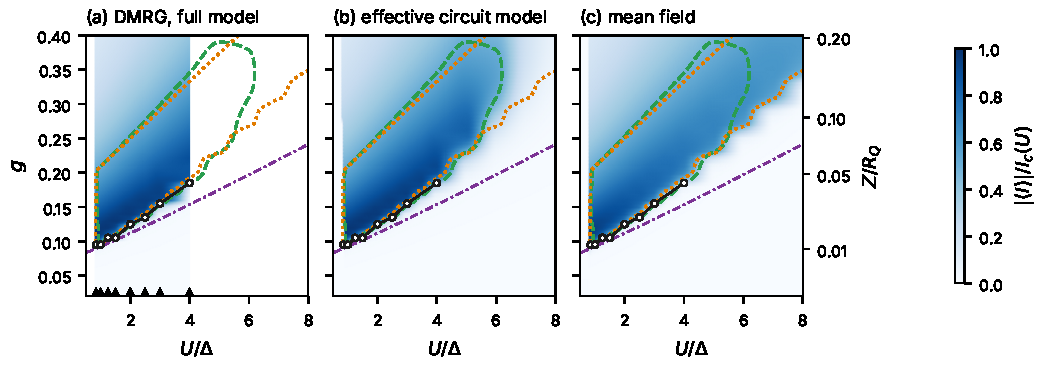
\includegraphics[width=\textwidth]{../figs/fig_phase_UG.pdf}
  \caption{\label{fig:phaseUG}%
  Phase diagram of the microscopic model~\eqref{eq:H} in the plane of the dot charging
  energy $U/\Delta$ and the mode coupling $g$ ($Z/R_Q=4g^2/\pi$, right axis), at
  $\hbar\omega=7.39\times10^{-4}\Delta$, $t_J=0.5\Delta$, $L=10$, no external flux
  (seed $\varphi_{\rm cl}=10^{-3}$). Colour: persistent current $|\langle I\rangle|$ from the
  gauge-invariant operator~\eqref{eq:Iop} in units of the junction critical current $I_c(U)$.
  (a) Full DMRG of electrons and photon (triangles: computed $U$ values; $g$ step $0.01$).
  (b) Effective circuit model $H_{\rm eff}$ with the DMRG $E(\varphi;U)$. (c) Mean field.
  Lines: contour $|\langle I\rangle|=0.5I_c$ from DMRG (solid), effective model (dashed) and
  mean field (dotted); white: classical threshold $\beta=1$.}
\end{figure*}

\begin{figure*}
  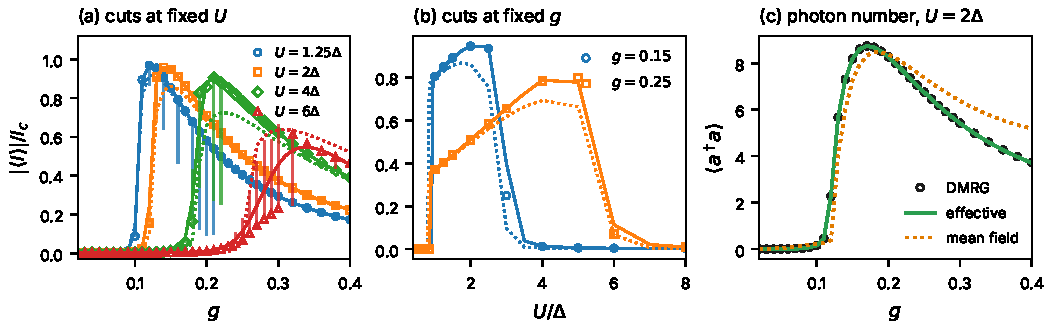
\includegraphics[width=\textwidth]{../figs/fig_phase_slices.pdf}
  \caption{\label{fig:phaseslices}%
  Cuts through Fig.~\ref{fig:phaseUG}. (a) Current versus $g$ at $U/\Delta=1.25,2,4$ and (b) versus
  $U$ at $g=0.15,0.25$: full DMRG (symbols), effective circuit model (solid), mean field (dotted).
  (c) Photon number at $U=2\Delta$.}
\end{figure*}

\begin{figure*}
  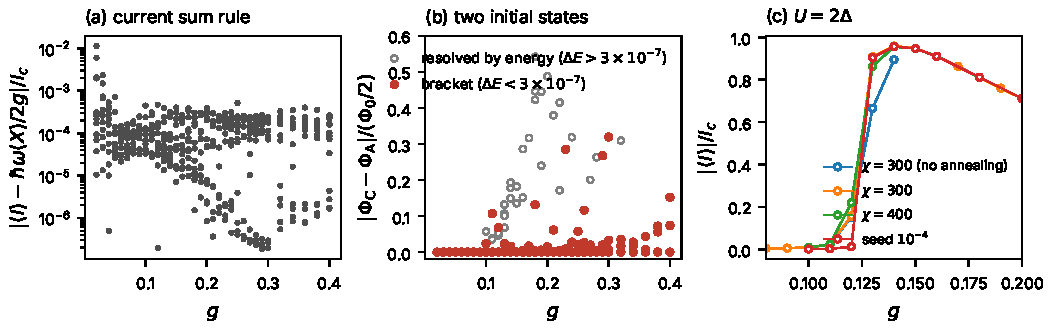
\includegraphics[width=\textwidth]{../figs/fig_phase_convergence.pdf}
  \caption{\label{fig:phaseconv}%
  Convergence of the full DMRG. (a) Violation of the sum rule~\eqref{eq:sumrule} over the whole
  grid. (b) Difference between the two initial states (vacuum side and polarized side) in units
  of $\Phi_0/2$. (c) $U=2\Delta$: bond dimension and seed dependence of the current near threshold.}
\end{figure*}

% ------------------------------------------------------------------
%  Results beyond the phase diagram: cat state of the pi loop (Fig. udot), half-flux-biased weak link
%  (Fig. halfflux), breakdown of the product state for E_J ~ hbar omega (Figs. notebook, notebook_omega).
%  Data: data/rerun/dmrg_udot_U2_Nr10_r10*.json, data/rerun/dmrg_weaklink_Nr14_r10_*.json (two-start protocol),
%  data/bo_udot_U2_Nr10.json, data/bo_weaklink.json; figures: code/make_figures.py
% ------------------------------------------------------------------

\paragraph*{Cat state and macroscopic tunnelling of the $\pi$ loop.}
Without a seed ($\varphi_{\rm cl}=0$ exactly) $H$ is real, $\langle I\rangle=0$ in every eigenstate, and the
order is diagnosed by the two lowest states of the doublet sector [Fig.~\ref{fig:udot}, $U=2\Delta$,
$E_J/\hbar\omega=10$, the parameters of the $U=2\Delta$ cut of Fig.~\ref{fig:phaseslices}].
The splitting $\delta=E_1-E_0$ collapses and the flux operator projected onto the quasi-degenerate
doublet acquires the eigenvalues $\pm\Phi^\star$. DMRG and the adiabatic theory give the same
$\Phi^\star$ to within $0.2\%$ at all $\beta$ [$\Phi^\star=0.59\,\Phi_0/2$ at $\beta=2$], the same photon
number to $0.03$, and the same
$\delta/\hbar\omega=0.70$, $0.24$ and $2.65\times10^{-4}$ at $\beta=0.5$, $1$ and $1.5$; at $\beta=1.5$ the
DMRG values at $\chi=300$ and $400$ are $2.66$ and $2.65\times10^{-4}$, so that the macroscopic tunnelling
of a condensate of seven photons ($\delta=2\times10^{-7}\Delta$) is resolved directly. Deeper in the ordered
phase $\delta$ drops below the DMRG resolution for excited-state energies ($4\times10^{-5}\,\hbar\omega$,
the change of the energies between $\chi=300$ and $400$); the adiabatic theory, validated above, then gives
$\delta/\hbar\omega=8\times10^{-7}$ and $7\times10^{-9}$ at $\beta=2$ and $3$. The exact ground-state
energy lies $(0.4$--$1.2)\times10^{-3}\hbar\omega$ above the adiabatic one, the non-adiabatic
correction of relative order $\hbar\omega/E_A$.
The seed-free DMRG ground state is the cat state itself: $|\langle\Phi\rangle|<10^{-3}\Phi^\star$, the flux
distribution $P(\Phi)$ is bimodal with peaks at $\pm\Phi^\star$ whose separation tracks the classical
minimum [Fig.~\ref{fig:udot}(c)], and a DMRG started from the polarized coherent state at $+\Phi^\star$
relaxes to the same symmetric state (energy difference $<10^{-10}\Delta$). This is the opposite situation
to the seeded scans of Fig.~\ref{fig:phaseUG}, where the seed selects one well and the two-start protocol
is needed to reach it. With increasing $E_J/\hbar\omega$ the crossover sharpens into a pitchfork at
$\beta=1$ and $\delta$ vanishes exponentially [Fig.~\ref{fig:udot}(b)]. The
residual $\delta$ is the macroscopic tunnelling of a persistent current. Because
it is protected by time-reversal symmetry, it is the only
energy scale separating the two current directions. Each current state is
additionally Kramers degenerate in the spin of the dot. The low-energy manifold is
therefore a fourfold multiplet $\{\sigma=\uparrow,\downarrow\}\otimes\{\circlearrowright,\circlearrowleft\}$,
split only by $\delta$.

\paragraph*{Half-flux-biased weak link.}
For an ordinary weak link ($L=14$, $t_J=0.5$, $E_2=-0.056\,\Delta$, $E_1=-5.4\times10^{-4}\Delta$, Andreev gap
$0.77\,\Delta$) biased by $\Phi_0/2$, Fig.~\ref{fig:halfflux} shows the full
DMRG solution at $E_J/\hbar\omega=10$ as a function of $\beta$, recomputed with the two-start protocol
(the sum rule~\eqref{eq:sumrule} holds to $2\times10^{-4}I_c$ at every point and to $6\times10^{-5}I_c$ above
threshold). The current
rises steeply at $\beta\simeq1.1$ and saturates at $|\langle I\rangle|\simeq0.96I_c$ for
$\beta\approx1.7$; the recomputed currents differ from the earlier warm-started runs by at most
$0.02I_c$ (at $\beta=1.1$--$1.4$), so this result was not affected by the under-polarization that
spoiled the seeded scans at the symmetric point. It then decreases as the flux approaches $\Phi_0/2$,
where the junction current vanishes. DMRG and the adiabatic theory agree to $2\times10^{-3}\hbar\omega$ in
energy, to $2\%$ of $I_c$ in current and to $1.3\%$ in $E_1-E_0$ at all $\beta$; the vacuum-side and
polarized-side starts give the same flux to $0.3\%$ and the same energy to $10^{-6}\Delta$, because the
tilt of the double well by the odd harmonic makes the landscape better conditioned than at the
symmetric point. The product state is
$0.2$--$0.4\hbar\omega$ too high in energy and overestimates the current
threefold near threshold ($0.71I_c$ versus $0.22I_c$ at $\beta=1.13$). It becomes accurate only deep in the
ordered phase, where the photon is a nearly coherent state.
The flux distribution extracted from the photon reduced density matrix
evolves from a Gaussian centred at zero to a single displaced peak at
$\pm\Phi^\star$. The sign is fixed by the residual odd harmonic
$E_1$, which tilts the double well by
$2|E_1|\sin\varphi^\star\approx10^{-3}\Delta\approx0.2\hbar\omega$.
This tilt sets the splitting $E_1-E_0$ for $\beta>1.2$ in DMRG and BO alike. Without it,
$\delta/\hbar\omega$ would drop below $10^{-6}$ at $\beta=2$. The external-bias
route thus provides a current-carrying state whose direction is \emph{selected}
rather than spontaneously chosen. Its residual symmetry breaking is
$\propto e^{-L/\xi}$ for a homogeneous ring, but in practice it is limited
by the flux offset $\delta\Phi$.

\paragraph*{Breakdown of the product-state description for $E_J\simeq\hbar\omega$.}
The product state is reliable only when $E_J\gg\hbar\omega$ and $g\ll1$, and both conditions are
violated by the parameters of the original mean-field solution~\cite{notebook}: a Zeeman-polarized
dot embedded in a short BCS ring ($t=2$, $\Delta=0.6$, $L=11$, $\epsilon_{d\uparrow}=-0.3$,
$\epsilon_{d\downarrow}=3.7$, $t_J=0.5$, $\hbar\omega=0.02$; energies in units of $t$ in this paragraph). The
self-consistent product state predicts a current-carrying phase for
$g\gtrsim0.75$, with $\langle a^\dagger a\rangle\simeq1$--$1.4$ and
$|\langle I\rangle|\approx0.02$ [Fig.~\ref{fig:notebook}]. DMRG shows that this
phase is an artefact. The exact ground-state energy decreases monotonically with
$g$ and lies below the MF energy by up to $1.8\hbar\omega$ (at $g=1.2$).
The gap to the first excited state stays a sizeable fraction of
$\hbar\omega$ ($E_1-E_0=0.33\hbar\omega$ at $g=1.2$), and the photon number
saturates at $\langle a^\dagger a\rangle\simeq0.36$. The response to the
seed flux $\varphi_{\rm cl}=10^{-3}$ is linear: $\langle I\rangle\approx7\times10^{-5}$,
more than two orders of magnitude below the MF value. DMRG and
the adiabatic theory~\eqref{eq:BO} agree to within $0.06\hbar\omega$ in
energy and $1.3\%$ in $E_1-E_0$. The residual difference is the non-adiabatic
(diagonal Born--Oppenheimer) correction, of relative order $\hbar\omega/E_A\approx0.1$.
At $\hbar\omega=0.002$ the same microscopic model does order, at
$g_c\simeq0.21$, while mean field predicts $g_c\simeq0.30$ [Fig.~\ref{fig:notebook_omega}].

Two effects make the product state fail. (i) It is not gauge invariant~\cite{Li2020,Dmytruk2021}: with the full
Peierls phase on one bond, it renormalizes that bond by
$|\langle D\rangle|<1$ and so loses phase-\emph{independent} kinetic energy,
which the exact state recovers by following the flux adiabatically. (ii) Here
$E_J\simeq\hbar\omega$. The Landau free energy does develop a double well
for $g>0.58$, but its depth is below the zero-point energy, and the flux
distribution $P(X)$ stays essentially unimodal. A further subtlety
concerns ring size: since $L\lesssim\xi$, $E(\varphi)$ of this ring is dominated by the
single-electron harmonic, $E_1=2.1\times10^{-2}\gg E_2=2.0\times10^{-3}$
[Fig.~\ref{fig:junctions}(a)]. The instability would then be one of the normal
$h/e$ persistent current rather than of the Josephson junction, which is why all
other results use rings with $L\gg\xi$.

% ------------------------------------------------------------------ figures
\begin{figure*}
  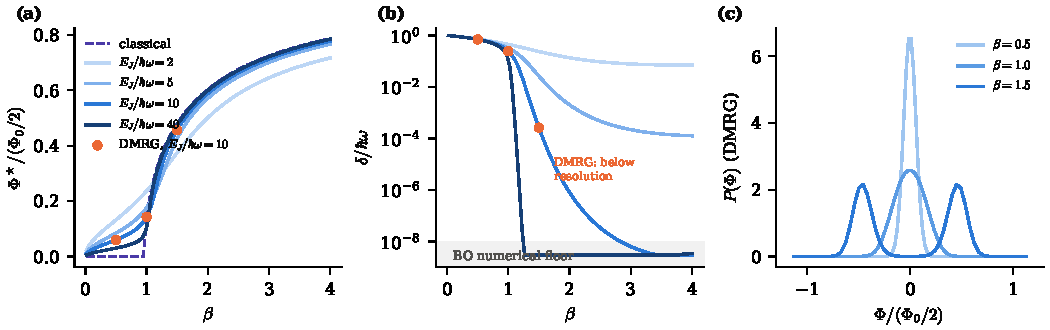
\includegraphics[width=\textwidth]{../figs/fig_udot_cavity.pdf}
  \caption{\label{fig:udot}%
  Interaction-driven $\pi$ loop ($U=2\Delta$, $L=10$, $\hbar\omega=E_J/10$, no external flux, no seed).
  (a) Flux of the condensate $\Phi^\star$ (eigenvalue of the flux projected on the two
  lowest states) versus $\beta$ for increasing $E_J/\hbar\omega$ (lines: adiabatic
  theory with the DMRG $E(\varphi)$; circles: full DMRG at $E_J/\hbar\omega=10$;
  dashed: classical). (b) Tunnel splitting $\delta$ between the two
  current-carrying states (triangles: DMRG below its resolution). (c) Flux distribution of the DMRG ground state
  (a cat state for $\beta>1$).}
\end{figure*}

\begin{figure*}
  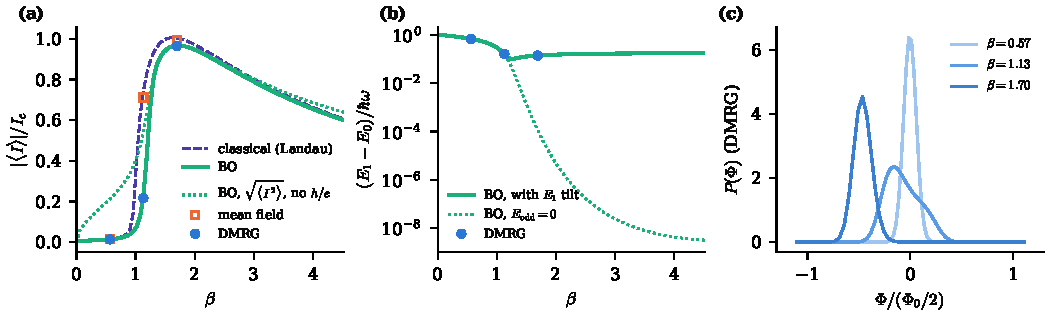
\includegraphics[width=\textwidth]{../figs/fig_weaklink_halfflux.pdf}
  \caption{\label{fig:halfflux}%
  Weak-link loop ($L=14$) biased by $\Phi_0/2$, $E_J/\hbar\omega=10$.
  (a) Persistent current, Eq.~\eqref{eq:Iop}, versus $\beta$: DMRG with the two-start protocol (circles),
  MF (squares), adiabatic theory with (solid) and without (dotted) the odd harmonics, classical
  Landau theory (dashed). (b) Splitting of the two lowest levels.
  (c) Flux distribution of the DMRG ground state, obtained from the photon reduced
  density matrix.}
\end{figure*}

\begin{figure}
  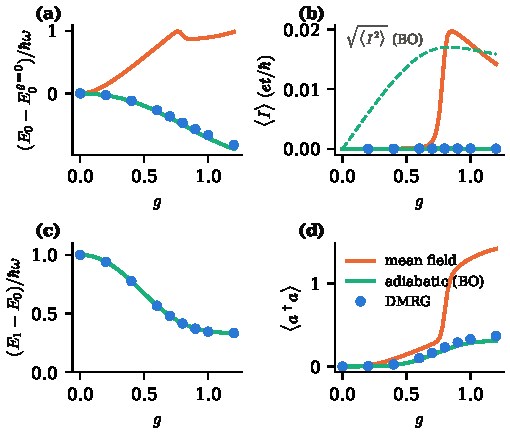
\includegraphics[width=\columnwidth]{../figs/fig_notebook_model.pdf}
  \caption{\label{fig:notebook}%
  Short ring with a Zeeman-polarized dot ($\hbar\omega=0.02$,
  $\varphi_{\rm cl}=10^{-3}$): mean field (MF, orange), adiabatic
  theory~\eqref{eq:BO} (green), and DMRG (symbols).
  (a) Ground-state energy, (b) current (dashed: rms current of the BO
  ground state), (c) gap to the first excited state, (d) photon number.}
\end{figure}

\begin{figure*}
  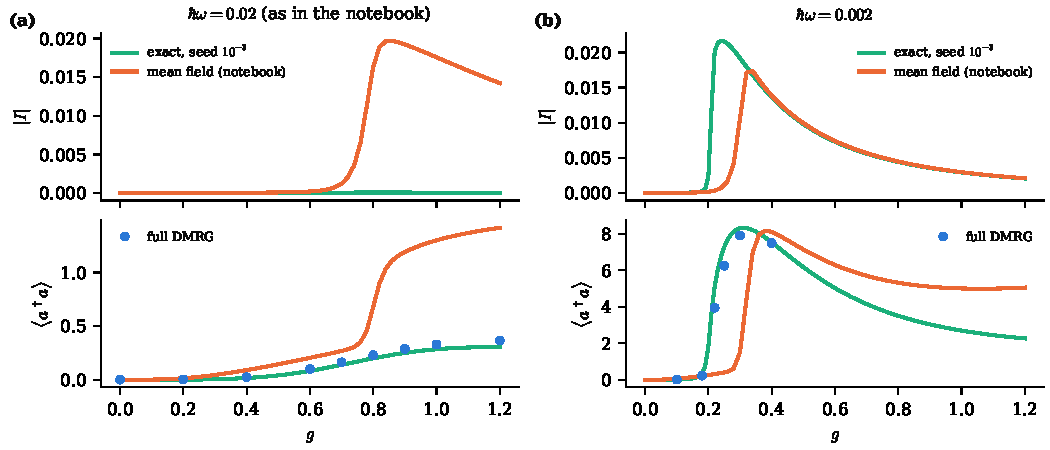
\includegraphics[width=\textwidth]{../figs/fig_notebook_omega.pdf}
  \caption{\label{fig:notebook_omega}%
  Model of the original notebook (Zeeman-polarized dot, $L=11$, $t=2$, $\Delta=0.6$):
  current (top) and photon number (bottom) versus $g$ for (a) $\hbar\omega=0.02$ and
  (b) $\hbar\omega=0.002$. Green: exact (adiabatic, seed $10^{-3}$); orange: mean field;
  circles: full DMRG (photon number; these older runs predate the two-start protocol).}
\end{figure*}


% ------------------------------------------------------------------
%  Section: the zero-point flux of the mode moves the 0-pi boundary (data/nonadiabatic, fig_cavity_0pi)
% ------------------------------------------------------------------
\paragraph*{Flux-driven $0$--$\pi$ switch.}
Figure~\ref{fig:cavity0pi} contains the first result. Without the mode the junction is a $0$ junction for
$U<U_c^0=0.94\Delta$, where the singlet is the ground state at zero flux, and a $\pi$ junction above (SM).
With the mode we compute the ground state of Eq.~\eqref{eq:H} in both parity sectors at $\varphi_{\rm cl}=0$,
without any seed, for $\hbar\omega=0.01$--$3\,\Delta$ and $g\le1$, and locate the boundary $U_c(g,\omega)$ of
the \emph{loop} from the crossing $E_{\rm odd}=E_{\rm even}$. At $U=0.9\Delta$ and $\hbar\omega=0.1\Delta$
[Fig.~\ref{fig:cavity0pi}(a)] the doublet--singlet energy difference falls from $+0.010\Delta$ at $g=0$ to
$-0.008\Delta$ at $g=0.4$ and $-0.065\Delta$ at $g=1$: the loop switches from $0$ to $\pi$ at $g\simeq0.28$,
a mode impedance $Z\simeq0.6\,{\rm k}\Omega$, with nothing but the vacuum of the mode acting on the junction.
The boundary $U_c(g,\omega)$ [Fig.~\ref{fig:cavity0pi}(b)] moves down at every $\omega$: to $0.83\Delta$ at
$g=0.5$ and to $0.65$, $0.60$ and $0.57\Delta$ at $g=1$ for $\hbar\omega=0.1$, $0.3$ and $1\,\Delta$, i.e.\ by
$30$--$40\%$ of $U_c^0$.

The mechanism changes with $\hbar\omega$. For $\hbar\omega\ll E_A$ the exact boundary coincides with that of
the circuit model~\eqref{eq:BO} (dashed; $0.889$ against $0.889\Delta$ at $g=0.4$ and $0.813$ against
$0.815\Delta$ at $g=0.8$ for $\hbar\omega=0.01\Delta$): the zero-point motion of the flux samples $E_s(gX)$
around $\varphi=0$, where the singlet surface curves up ($E''_{\rm even}(0)=+0.20\Delta$) and the doublet
surface curves down, so that the singlet loses and the doublet gains zero-point energy,
$\delta E_s\simeq\tfrac12g^2E''_s(0)\langle X^2\rangle$, and for $gX$ of order one the doublet lowers its
energy further by letting the flux relax towards $\Phi_0/2$, where its minimum lies. This is the quantum
version of the parity switch by a free flux discussed below. As $\hbar\omega$ grows the exact boundary
leaves the circuit model (by $0.015$, $0.032$ and $0.040\Delta$ at $g=0.8$ for $\hbar\omega=0.1$, $0.3$ and
$1\,\Delta$) and settles on the Lang--Firsov line (dotted) at $\hbar\omega\simeq\Delta$: $0.663$ against
$0.670\Delta$ at $g=0.8$, and $\hbar\omega=3\Delta$ gives the same boundary to $10^{-3}\Delta$. There the mode no
longer follows the junction but reduces the level width of the dressed bond by $e^{-g^2}$, and the singlet,
which is bound by $\Gamma$, loses against the doublet. The adiabatic shift is bounded by the condensation
energy of the $\pi$ well, the Franck--Condon shift by $\Gamma$ alone, and the corrections $O(t_J^2/\hbar\omega)$
are below $0.01\Delta$ at $\hbar\omega=\Delta$. The dressing of the
junction is visible in the Peierls factor and in the photon--electron entanglement
[Fig.~\ref{fig:cavity0pi}(c)]: $|\langle D\rangle|$ follows $e^{-g^2/2}$ for $\hbar\omega\gtrsim0.3\Delta$,
where the mode is only squeezed by its vacuum, and falls faster in the adiabatic regime, where it is
displaced towards the $\pi$ well; the entanglement entropy is largest there ($0.26$ at $g=0.8$,
$\hbar\omega=0.01\Delta$), because the flux state depends on the electronic sector.

The effect is not an artefact of the one-bond vertex: the neglected capacitive terms are of relative order
$\hbar\omega g^2/E_A$, and the shift of $U_c$ at $\hbar\omega=0.01\Delta$, where they are negligible, is
already half of the one at $\hbar\omega=0.3\Delta$. Nor is it a mean-field effect: the Hartree--Fock product
state replaces the Kramers doublet by a static moment and places the boundary at $0.82\Delta$ for every $g$
(next section). The prediction is that a dot junction gate tuned close to its singlet--doublet boundary, in a loop
whose inductance is a superinductor of impedance $Z\gtrsim1\,{\rm k}\Omega$, is driven into the $\pi$ phase
by the impedance alone, with the switch visible as the jump of the resonator frequency that marks the parity
transition in Refs.~\cite{Bargerbos2022,PitaVidal2023}.

\begin{figure*}
  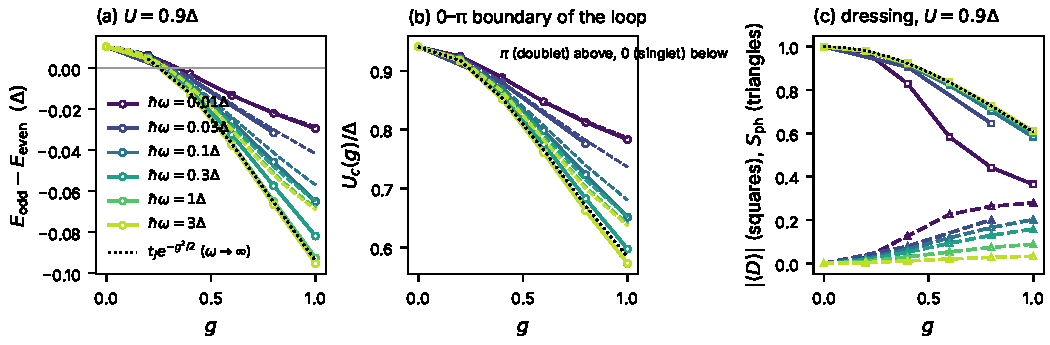
\includegraphics[width=\textwidth]{../figs/fig_cavity_0pi.pdf}
  \caption{\label{fig:cavity0pi}%
  Zero-point flux and the $0$--$\pi$ transition ($L=10$, $t_J=0.5\Delta$, $\varphi_{\rm cl}=0$, no seed).
  (a) Doublet--singlet energy difference versus $g$ at $U=0.9\Delta$ for $\hbar\omega=0.01$--$3\,\Delta$: full
  DMRG (symbols), circuit model~\eqref{eq:BO} with the $g=0$ surfaces (dashed), Lang--Firsov ring with
  $t_Je^{-g^2/2}$ on the dressed bond (dotted, the $\omega\to\infty$ limit). The sign change is the switch of the loop from $0$ to $\pi$.
  (b) Boundary $U_c(g,\omega)$ of the loop from the crossing $E_{\rm odd}=E_{\rm even}$ (same symbols and lines).
  (c) Dressing of the junction in the doublet sector at $U=0.9\Delta$: $|\langle D\rangle|$ (squares; dotted:
  $e^{-g^2/2}$) and the photon--electron entanglement entropy $S_{\rm ph}$ (triangles).}
\end{figure*}

% ------------------------------------------------------------------
%  Section: exact (U, g) phase diagram of the microscopic model
%  Full DMRG of Eq. (H) vs effective circuit model vs mean field.
%  Numbers marked \TODO are filled from data/full, data/effective_Nr10.json, data/mf_grid_Nr10.json.
% ------------------------------------------------------------------

\paragraph*{Choice of regime and dimensionless variables.}
The microscopic model~\eqref{eq:H} contains the energy scales $t,\Delta,t_J,U$
of the junction and $\hbar\omega,g$ of the mode. Three dimensionless ratios
control the physics. (i) $U/\Delta$ at fixed $\Gamma/\Delta$ (here $\Gamma=2t_J^2/t=\Delta/2$)
sets the magnetic state of the dot and hence the sign of the Josephson coupling:
the loop is a $\pi$ loop only for $U>U_c$. (ii) The coupling $g$ is fixed by
the impedance of the mode alone, $g^2=\pi Z/4R_Q$, i.e.\ $g=0.1$--$0.4$
for $Z=0.08$--$1.3\,{\rm k}\Omega$, the range of superinducting resonators~\cite{Manucharyan2009,Grunhaupt2019}.
(iii) $E_J/\hbar\omega$, with $E_J\equiv E_2>0$ the Josephson energy of the $\pi$ junction,
decides whether the transition is sharp: the two current states tunnel with
$\delta\sim\hbar\omega e^{-S}$, $S\propto E_J/\hbar\omega$. We take
$\hbar\omega=E_J(U=2\Delta)/10=7.39\times10^{-4}\Delta$: for a dot junction with
$I_c^\pi\simeq10$\,nA ($E_J/h\simeq5$\,GHz) this is a $500$\,MHz mode, as realized by
a loop of superinductance $L\simeq\Phi_0/2\pi I_c\simeq 30\,\mu$H--equivalently a
fluxonium-type circuit~\cite{Manucharyan2009}. With this choice the classical threshold
$\beta=8g^2E_J(U)/\hbar\omega=1$ lies at $g_c=0.11$ for $U=2\Delta$ and
sweeps across the experimentally accessible window $g\le0.4$ as $U$ is varied
from $U_c$ to $8\Delta$, while $E_J/\hbar\omega\ge5$ keeps the ordered phase
well defined ($\delta/\hbar\omega<10^{-2}$ for $\beta>1.3$). We present the phase diagram in the
plane $(U/\Delta,g)$; the right axis of Fig.~\ref{fig:phaseUG} converts $g$ to $Z/R_Q$.
The ring has $L=10$ sites ($L\gg\xi\simeq t/\Delta$): the $\pi$-sector Josephson
energy is converged to $0.2\%$ between $L=8$ and $L=14$
($E_2=7.403,7.392,7.391,7.391\times10^{-3}\Delta$ for $L=8,10,12,14$) and the single-electron
harmonic is $|E_1|/E_2\le2\%$.

\paragraph*{Gauge-invariant current operator.}
Since the Peierls phase of the loop is placed on the dot--ring bond (Eq.~\eqref{eq:H}),
the persistent current is the derivative of $H$ with respect to the total flux,
$I=-(2e/\hbar)\,\partial H/\partial\varphi_{\rm cl}$,
\begin{equation}
  I=\frac{2e}{\hbar}\,i\,t_J\sum_\sigma\!\left(e^{i\varphi_{\rm cl}}e^{ig(a+a^\dagger)}c^\dagger_{1\sigma}c_{0\sigma}
  -{\rm h.c.}\right)
  \label{eq:Iop}
\end{equation}
(below we quote $I$ in units of $2e\Delta/\hbar$). This is the particle current through the
dot--ring bond, dressed by the displacement operator of the mode: the combination
$e^{i(\varphi_{\rm cl}+gX)}c^\dagger_1c_0$ is invariant under the simultaneous
gauge transformation of the electrons and of the vector potential, and its
expectation value does not change if the Peierls phase is distributed along the
ring with the pairing amplitude transformed covariantly~\cite{Dmytruk2021}.
Because the dot carries no pairing term, the particle number of site $0$ is conserved by
$H$ and the current entering the dot from site $L-1$ equals the current~\eqref{eq:Iop}
leaving it; the same is not true of the bonds inside the BCS chain, where the
fixed-phase pairing term acts as a condensate reservoir~\cite{Dmytruk2021}.
Equation~\eqref{eq:Iop} obeys an exact sum rule. With $X=a+a^\dagger$ and
$P=-i(a-a^\dagger)$, $[H,P]=i\hbar\omega X-2ig\,(\hbar/2e)I$, so that in any eigenstate
\begin{equation}
  \langle I\rangle=\frac{2e}{\hbar}\,\frac{\hbar\omega}{2g}\,\langle a+a^\dagger\rangle ,
  \label{eq:sumrule}
\end{equation}
the persistent current \emph{is} the static displacement of the mode (the dc flux
it generates, $\Phi=L I$). We evaluate both sides independently in DMRG and use their
difference as a convergence measure: $\langle I\rangle$ is a local fermionic observable,
$\langle X\rangle$ a photonic one, and only an eigenstate satisfies Eq.~\eqref{eq:sumrule}.

\paragraph*{DMRG protocol.}
At each $(U,g)$ we obtain the ground state of Eq.~\eqref{eq:H} on the full
electron--photon Hilbert space by two-site DMRG with bond dimension $\chi=300$
(truncation error $<10^{-9}$), a photon cutoff $N_{\rm ph}=50$--$90$ chosen such that
the population of the last Fock state is $<10^{-8}$, and a seed
$\varphi_{\rm cl}=10^{-3}$ that selects one of the two degenerate current states. Fermion
parity and $S^z$ are conserved; both parity sectors are computed and the lower one is
taken, which locates the $0$--$\pi$ boundary without any assumption. The two current-carrying states
are split only by the exponentially small $\delta$ and by the seed, $2I^\star\varphi_{\rm cl}\sim10^{-5}\Delta$,
so that the energy landscape between them is flat and local DMRG updates converge slowly
towards the polarized state. We therefore use two independent initial states at every
point and keep the lower-energy result: (A) the converged state of the neighbouring $g$,
which approaches the transition from the vacuum side, and (C) a product state with the
mode in a coherent state at the classical flux, converged first with a large seed
($\varphi_{\rm cl}=10^{-2}$, then $3\times10^{-3}$) and then relaxed at $10^{-3}$, which
approaches it from the polarized side. Away from the threshold the two agree
to $\Delta\langle X\rangle<\TODO{}$; in a window $\Delta g\lesssim0.01$ around $g_c$ they bracket the
exact result (the ground state there is a partially polarized cat, and the DMRG error bar is
the bracket). The sum rule~\eqref{eq:sumrule} is satisfied to better than
$\TODO{}\,I_c$ at every point of the grid [Fig.~\ref{fig:phaseconv}(a)].

\paragraph*{Effective circuit model.}
When $\hbar\omega$ is small compared to the Andreev gap $E_A$ of the junction
($\hbar\omega/E_A\simeq10^{-3}$ here), the fermions can be integrated out
adiabatically: the mode moves in the exact ground-state energy of the ring at fixed phase,
$H_{\rm eff}=\hbar\omega a^\dagger a+E(\varphi_{\rm cl}+gX;U)$ [Eq.~\eqref{eq:BO}], i.e.\ an rf-SQUID
Hamiltonian with the inductive energy supplied by the mode. The matching of parameters
is unambiguous: $E(\varphi;U)$ is computed by DMRG at $g=0$ in both parity sectors on
$\varphi\in[0,\pi]$ and represented by four harmonics (the lower sector is taken point by point,
so the level crossing of the $0'$ and $\pi'$ regions is kept). $H_{\rm eff}$ is then diagonalized
exactly in a Fock space of $200$ states, with the same seed. Its current is
$I_{\rm eff}=-(2e/\hbar)\partial_\varphi E$, the classical current of the junction averaged over the flux
distribution of the mode; the omitted terms are the non-adiabatic (Berry) corrections of relative
order $\hbar\omega/E_A$. The mean-field theory of Ref.~\cite{notebook}, generalized to the
interacting dot (Hartree--Fock BdG electrons $\times$ photon product state, swept upwards in $g$
with the same seed), is evaluated on the same grid.

\paragraph*{Phase diagram.}
Figure~\ref{fig:phaseUG} shows $|\langle I\rangle|/I_c(U)$, with $I_c(U)$ the critical current of
the $\pi$ junction at $g=0$, from the full DMRG (a), the effective circuit model (b) and mean field (c);
Fig.~\ref{fig:phaseslices} shows cuts. The exact diagram has three regions.
(i) For $U<U_c^{\pi'}=\TODO{0.83}\Delta$ the ground state of the loop is the singlet $0$ junction at every
flux, the orbital response is diamagnetic and the mode stays in its vacuum for all
$g\le0.4$ ($\langle a^\dagger a\rangle<\TODO{}$, $|\langle I\rangle|<\TODO{}I_c$, linear in the seed).
(ii) For $U>U_c^{\pi'}$ and $g>g_c(U)$ the mode condenses: at $U=2\Delta$ the photon number rises from
$0.5$ at $g=0.11$ to $5.7$ at $g=0.13$ and $7.3$ at $g=0.14$, where the current reaches
$0.96\,I_c$; it then decreases as $I\simeq(2e/\hbar)\hbar\omega\varphi^\star/2g^2$, because the condensate
flux saturates at $\Phi_0/2$ while the inductance $\propto g^2/\hbar\omega$ grows [Eq.~\eqref{eq:sumrule}].
The threshold $g_c(U)$ (contour $|\langle I\rangle|=0.5I_c$) rises from $0.10$ at $U=\Delta$ to $0.13$, $0.19$ and $0.31$ at
$U=2,4,6\Delta$, following the decrease of $E_J(U)$. It lies systematically \emph{above} the classical
line $\beta=1$ (white), by $\Delta g=0.02$ at $U=2\Delta$ and $0.11$ at $U=6\Delta$: the zero-point
motion of the flux opposes the condensation, and the shift grows as $E_J/\hbar\omega$ decreases
from $10$ to $3.2$. For $U\ge7\Delta$ ($E_J/\hbar\omega\le2.6$) the ordered phase has disappeared
from the window $g\le0.4$ although $\beta$ reaches $3.3$: there the ground state is the cat state
with $\delta\simeq\hbar\omega$ and $\langle I\rangle\to0$ as the seed is removed, the finite-$E_J/\hbar\omega$
remnant of the transition.
(iii) In the window $U_c^{\pi'}<U<U_c^{0}=\TODO{0.94}\Delta$ the singlet is the ground state at zero flux but the
doublet, whose energy minimum lies at $\varphi=\pi/2$, is lower by up to \TODO{}$\Delta$ once the flux is
allowed to adjust: the mode drives the parity switch and the loop orders with the full $\pi$-junction
current, at a threshold that moves to larger $g$ as $U\to U_c^{\pi'}$ [\TODO{DMRG numbers for U=0.85}].
The $0$--$\pi$ boundary of the loop is therefore not the zero-flux crossing $U_c^0$ of the junction
but the crossing of the global minima, $U_c^{\pi'}$, and it is essentially independent of $g$
(the condensation energy, $\lesssim E_J/4\simeq2\times10^{-3}\Delta$, shifts it by $<0.01\Delta$).

\paragraph*{Comparison with the effective model and with mean field.}
Above threshold the full DMRG and the effective circuit model agree to $0.3\%$ in the current and
to $0.1$ in the photon number at $U=2\Delta$ (and to $\TODO{}\%$ over the whole ordered region),
which validates the adiabatic elimination of the fermions at $\hbar\omega/E_A\sim10^{-3}$. The only
points where they differ by more are the single crossover point per $U$ ($g=0.12$ at $U=2\Delta$,
$g=0.14$ at $U=2.5\Delta$), where the exact ground state is a partially polarized cat and the
DMRG bracket from the two initial states is wide [Fig.~\ref{fig:phaseconv}(b)]. This is a statement
about the convergence of a variational method on a flat energy landscape, not about the physics:
the energy difference between the two starts is $<3\times10^{-6}\Delta$, while the effective model,
which resolves it exactly, interpolates smoothly between them. Mean field locates $g_c(U)$ to within
the grid step $0.01$ for $U\le4\Delta$, but underestimates the current by $10$--$20\%$
($0.86$ versus $0.96\,I_c$ at $U=2\Delta$; $0.82$ versus $0.95\,I_c$ at $2.5\Delta$) because the product
state renormalizes the junction bond by $|\langle D\rangle|<1$; it overestimates the photon number at
large $g$ ($5.3$ versus $3.7$ at $U=2\Delta$, $g=0.4$), where the exact flux distribution is a displaced
squeezed state rather than a coherent state; and it predicts an ordered phase at $U=7$--$8\Delta$ that
the exact solution does not have, because a product state cannot describe the tunnelling between the
two current directions that restores the symmetry when $E_J\lesssim3\hbar\omega$. Its threshold
$U_c^{\rm MF}=0.82\Delta$ coincides with $U_c^{\pi'}$ only accidentally: in Hartree--Fock the dot
becomes a static moment, whereas the exact doublet is a Kramers pair.

\begin{figure*}
  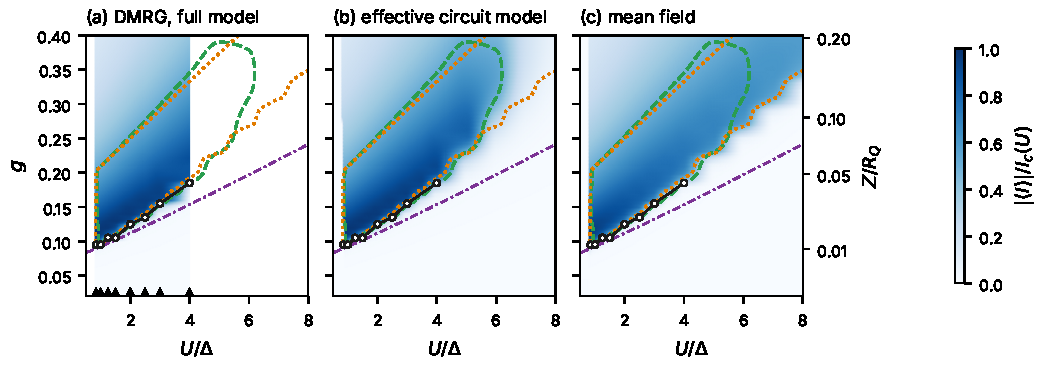
\includegraphics[width=\textwidth]{../figs/fig_phase_UG.pdf}
  \caption{\label{fig:phaseUG}%
  Phase diagram of the microscopic model~\eqref{eq:H} in the plane of the dot charging
  energy $U/\Delta$ and the mode coupling $g$ ($Z/R_Q=4g^2/\pi$, right axis), at
  $\hbar\omega=7.39\times10^{-4}\Delta$, $t_J=0.5\Delta$, $L=10$, no external flux
  (seed $\varphi_{\rm cl}=10^{-3}$). Colour: persistent current $|\langle I\rangle|$ from the
  gauge-invariant operator~\eqref{eq:Iop} in units of the junction critical current $I_c(U)$.
  (a) Full DMRG of electrons and photon (triangles: computed $U$ values; $g$ step $0.01$).
  (b) Effective circuit model $H_{\rm eff}$ with the DMRG $E(\varphi;U)$. (c) Mean field.
  Lines: contour $|\langle I\rangle|=0.5I_c$ from DMRG (solid), effective model (dashed) and
  mean field (dotted); white: classical threshold $\beta=1$.}
\end{figure*}

\begin{figure*}
  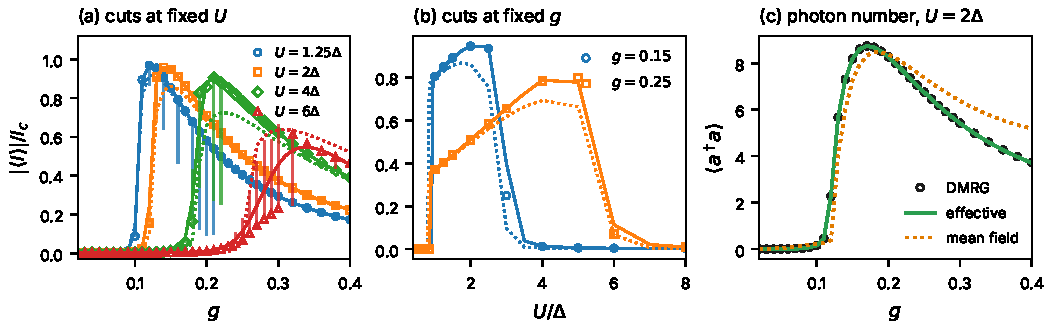
\includegraphics[width=\textwidth]{../figs/fig_phase_slices.pdf}
  \caption{\label{fig:phaseslices}%
  Cuts through Fig.~\ref{fig:phaseUG}. (a) Current versus $g$ at $U/\Delta=1.25,2,4$ and (b) versus
  $U$ at $g=0.15,0.25$: full DMRG (symbols), effective circuit model (solid), mean field (dotted).
  (c) Photon number at $U=2\Delta$.}
\end{figure*}

\begin{figure*}
  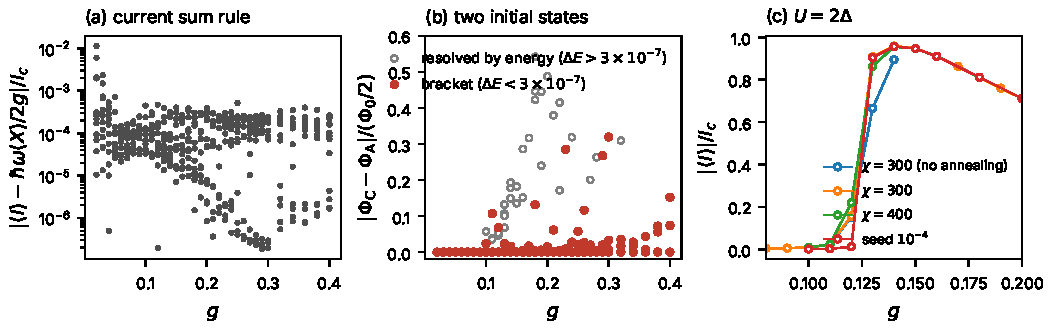
\includegraphics[width=\textwidth]{../figs/fig_phase_convergence.pdf}
  \caption{\label{fig:phaseconv}%
  Convergence of the full DMRG. (a) Violation of the sum rule~\eqref{eq:sumrule} over the whole
  grid. (b) Difference between the two initial states (vacuum side and polarized side) in units
  of $\Phi_0/2$. (c) $U=2\Delta$: bond dimension and seed dependence of the current near threshold.}
\end{figure*}

% ------------------------------------------------------------------
%  Results beyond the phase diagram: cat state of the pi loop (Fig. udot), half-flux-biased weak link
%  (Fig. halfflux), breakdown of the product state for E_J ~ hbar omega (Figs. notebook, notebook_omega).
%  Data: data/rerun/dmrg_udot_U2_Nr10_r10*.json, data/rerun/dmrg_weaklink_Nr14_r10_*.json (two-start protocol),
%  data/bo_udot_U2_Nr10.json, data/bo_weaklink.json; figures: code/make_figures.py
% ------------------------------------------------------------------

\paragraph*{Cat state and macroscopic tunnelling of the $\pi$ loop.}
Without a seed ($\varphi_{\rm cl}=0$ exactly) $H$ is real, $\langle I\rangle=0$ in every eigenstate, and the
order is diagnosed by the two lowest states of the doublet sector [Fig.~\ref{fig:udot}, $U=2\Delta$,
$E_J/\hbar\omega=10$, the parameters of the $U=2\Delta$ cut of Fig.~\ref{fig:phaseslices}].
The splitting $\delta=E_1-E_0$ collapses and the flux operator projected onto the quasi-degenerate
doublet acquires the eigenvalues $\pm\Phi^\star$. DMRG and the adiabatic theory give the same
$\Phi^\star$ to within $0.2\%$ at all $\beta$ [$\Phi^\star=0.59\,\Phi_0/2$ at $\beta=2$], the same photon
number to $0.03$, and the same
$\delta/\hbar\omega=0.70$, $0.24$ and $2.65\times10^{-4}$ at $\beta=0.5$, $1$ and $1.5$; at $\beta=1.5$ the
DMRG values at $\chi=300$ and $400$ are $2.66$ and $2.65\times10^{-4}$, so that the macroscopic tunnelling
of a condensate of seven photons ($\delta=2\times10^{-7}\Delta$) is resolved directly. Deeper in the ordered
phase $\delta$ drops below the DMRG resolution for excited-state energies ($4\times10^{-5}\,\hbar\omega$,
the change of the energies between $\chi=300$ and $400$); the adiabatic theory, validated above, then gives
$\delta/\hbar\omega=8\times10^{-7}$ and $7\times10^{-9}$ at $\beta=2$ and $3$. The exact ground-state
energy lies $(0.4$--$1.2)\times10^{-3}\hbar\omega$ above the adiabatic one, the non-adiabatic
correction of relative order $\hbar\omega/E_A$.
The seed-free DMRG ground state is the cat state itself: $|\langle\Phi\rangle|<10^{-3}\Phi^\star$, the flux
distribution $P(\Phi)$ is bimodal with peaks at $\pm\Phi^\star$ whose separation tracks the classical
minimum [Fig.~\ref{fig:udot}(c)], and a DMRG started from the polarized coherent state at $+\Phi^\star$
relaxes to the same symmetric state (energy difference $<10^{-10}\Delta$). This is the opposite situation
to the seeded scans of Fig.~\ref{fig:phaseUG}, where the seed selects one well and the two-start protocol
is needed to reach it. With increasing $E_J/\hbar\omega$ the crossover sharpens into a pitchfork at
$\beta=1$ and $\delta$ vanishes exponentially [Fig.~\ref{fig:udot}(b)]. The
residual $\delta$ is the macroscopic tunnelling of a persistent current. Because
it is protected by time-reversal symmetry, it is the only
energy scale separating the two current directions. Each current state is
additionally Kramers degenerate in the spin of the dot. The low-energy manifold is
therefore a fourfold multiplet $\{\sigma=\uparrow,\downarrow\}\otimes\{\circlearrowright,\circlearrowleft\}$,
split only by $\delta$.

\paragraph*{Half-flux-biased weak link.}
For an ordinary weak link ($L=14$, $t_J=0.5$, $E_2=-0.056\,\Delta$, $E_1=-5.4\times10^{-4}\Delta$, Andreev gap
$0.77\,\Delta$) biased by $\Phi_0/2$, Fig.~\ref{fig:halfflux} shows the full
DMRG solution at $E_J/\hbar\omega=10$ as a function of $\beta$, recomputed with the two-start protocol
(the sum rule~\eqref{eq:sumrule} holds to $2\times10^{-4}I_c$ at every point and to $6\times10^{-5}I_c$ above
threshold). The current
rises steeply at $\beta\simeq1.1$ and saturates at $|\langle I\rangle|\simeq0.96I_c$ for
$\beta\approx1.7$; the recomputed currents differ from the earlier warm-started runs by at most
$0.02I_c$ (at $\beta=1.1$--$1.4$), so this result was not affected by the under-polarization that
spoiled the seeded scans at the symmetric point. It then decreases as the flux approaches $\Phi_0/2$,
where the junction current vanishes. DMRG and the adiabatic theory agree to $2\times10^{-3}\hbar\omega$ in
energy, to $2\%$ of $I_c$ in current and to $1.3\%$ in $E_1-E_0$ at all $\beta$; the vacuum-side and
polarized-side starts give the same flux to $0.3\%$ and the same energy to $10^{-6}\Delta$, because the
tilt of the double well by the odd harmonic makes the landscape better conditioned than at the
symmetric point. The product state is
$0.2$--$0.4\hbar\omega$ too high in energy and overestimates the current
threefold near threshold ($0.71I_c$ versus $0.22I_c$ at $\beta=1.13$). It becomes accurate only deep in the
ordered phase, where the photon is a nearly coherent state.
The flux distribution extracted from the photon reduced density matrix
evolves from a Gaussian centred at zero to a single displaced peak at
$\pm\Phi^\star$. The sign is fixed by the residual odd harmonic
$E_1$, which tilts the double well by
$2|E_1|\sin\varphi^\star\approx10^{-3}\Delta\approx0.2\hbar\omega$.
This tilt sets the splitting $E_1-E_0$ for $\beta>1.2$ in DMRG and BO alike. Without it,
$\delta/\hbar\omega$ would drop below $10^{-6}$ at $\beta=2$. The external-bias
route thus provides a current-carrying state whose direction is \emph{selected}
rather than spontaneously chosen. Its residual symmetry breaking is
$\propto e^{-L/\xi}$ for a homogeneous ring, but in practice it is limited
by the flux offset $\delta\Phi$.

\paragraph*{Breakdown of the product-state description for $E_J\simeq\hbar\omega$.}
The product state is reliable only when $E_J\gg\hbar\omega$ and $g\ll1$, and both conditions are
violated by the parameters of the original mean-field solution~\cite{notebook}: a Zeeman-polarized
dot embedded in a short BCS ring ($t=2$, $\Delta=0.6$, $L=11$, $\epsilon_{d\uparrow}=-0.3$,
$\epsilon_{d\downarrow}=3.7$, $t_J=0.5$, $\hbar\omega=0.02$; energies in units of $t$ in this paragraph). The
self-consistent product state predicts a current-carrying phase for
$g\gtrsim0.75$, with $\langle a^\dagger a\rangle\simeq1$--$1.4$ and
$|\langle I\rangle|\approx0.02$ [Fig.~\ref{fig:notebook}]. DMRG shows that this
phase is an artefact. The exact ground-state energy decreases monotonically with
$g$ and lies below the MF energy by up to $1.8\hbar\omega$ (at $g=1.2$).
The gap to the first excited state stays a sizeable fraction of
$\hbar\omega$ ($E_1-E_0=0.33\hbar\omega$ at $g=1.2$), and the photon number
saturates at $\langle a^\dagger a\rangle\simeq0.36$. The response to the
seed flux $\varphi_{\rm cl}=10^{-3}$ is linear: $\langle I\rangle\approx7\times10^{-5}$,
more than two orders of magnitude below the MF value. DMRG and
the adiabatic theory~\eqref{eq:BO} agree to within $0.06\hbar\omega$ in
energy and $1.3\%$ in $E_1-E_0$. The residual difference is the non-adiabatic
(diagonal Born--Oppenheimer) correction, of relative order $\hbar\omega/E_A\approx0.1$.
At $\hbar\omega=0.002$ the same microscopic model does order, at
$g_c\simeq0.21$, while mean field predicts $g_c\simeq0.30$ [Fig.~\ref{fig:notebook_omega}].

Two effects make the product state fail. (i) It is not gauge invariant~\cite{Li2020,Dmytruk2021}: with the full
Peierls phase on one bond, it renormalizes that bond by
$|\langle D\rangle|<1$ and so loses phase-\emph{independent} kinetic energy,
which the exact state recovers by following the flux adiabatically. (ii) Here
$E_J\simeq\hbar\omega$. The Landau free energy does develop a double well
for $g>0.58$, but its depth is below the zero-point energy, and the flux
distribution $P(X)$ stays essentially unimodal. A further subtlety
concerns ring size: since $L\lesssim\xi$, $E(\varphi)$ of this ring is dominated by the
single-electron harmonic, $E_1=2.1\times10^{-2}\gg E_2=2.0\times10^{-3}$
[Fig.~\ref{fig:junctions}(a)]. The instability would then be one of the normal
$h/e$ persistent current rather than of the Josephson junction, which is why all
other results use rings with $L\gg\xi$.

% ------------------------------------------------------------------ figures
\begin{figure*}
  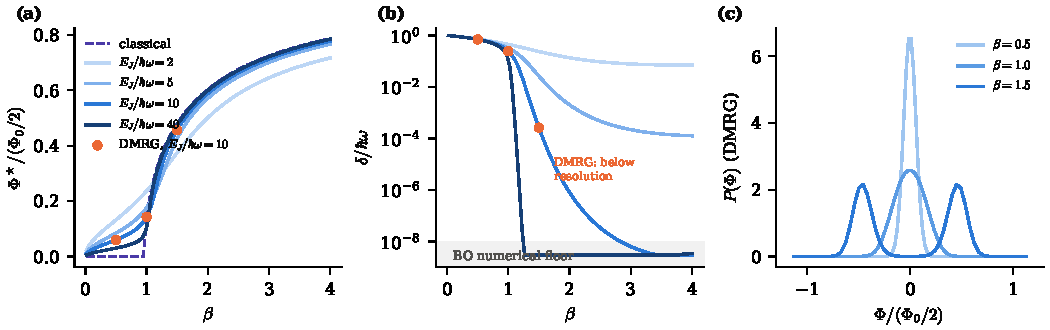
\includegraphics[width=\textwidth]{../figs/fig_udot_cavity.pdf}
  \caption{\label{fig:udot}%
  Interaction-driven $\pi$ loop ($U=2\Delta$, $L=10$, $\hbar\omega=E_J/10$, no external flux, no seed).
  (a) Flux of the condensate $\Phi^\star$ (eigenvalue of the flux projected on the two
  lowest states) versus $\beta$ for increasing $E_J/\hbar\omega$ (lines: adiabatic
  theory with the DMRG $E(\varphi)$; circles: full DMRG at $E_J/\hbar\omega=10$;
  dashed: classical). (b) Tunnel splitting $\delta$ between the two
  current-carrying states (triangles: DMRG below its resolution). (c) Flux distribution of the DMRG ground state
  (a cat state for $\beta>1$).}
\end{figure*}

\begin{figure*}
  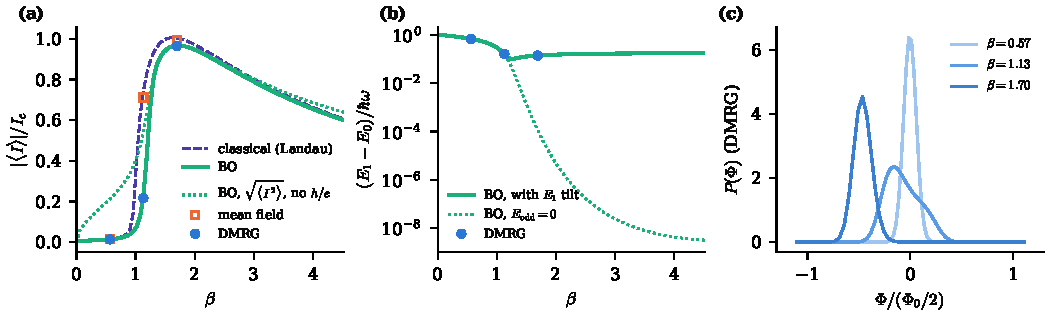
\includegraphics[width=\textwidth]{../figs/fig_weaklink_halfflux.pdf}
  \caption{\label{fig:halfflux}%
  Weak-link loop ($L=14$) biased by $\Phi_0/2$, $E_J/\hbar\omega=10$.
  (a) Persistent current, Eq.~\eqref{eq:Iop}, versus $\beta$: DMRG with the two-start protocol (circles),
  MF (squares), adiabatic theory with (solid) and without (dotted) the odd harmonics, classical
  Landau theory (dashed). (b) Splitting of the two lowest levels.
  (c) Flux distribution of the DMRG ground state, obtained from the photon reduced
  density matrix.}
\end{figure*}

\begin{figure}
  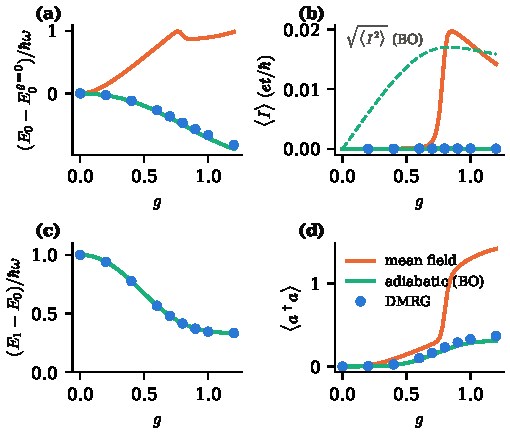
\includegraphics[width=\columnwidth]{../figs/fig_notebook_model.pdf}
  \caption{\label{fig:notebook}%
  Short ring with a Zeeman-polarized dot ($\hbar\omega=0.02$,
  $\varphi_{\rm cl}=10^{-3}$): mean field (MF, orange), adiabatic
  theory~\eqref{eq:BO} (green), and DMRG (symbols).
  (a) Ground-state energy, (b) current (dashed: rms current of the BO
  ground state), (c) gap to the first excited state, (d) photon number.}
\end{figure}

\begin{figure*}
  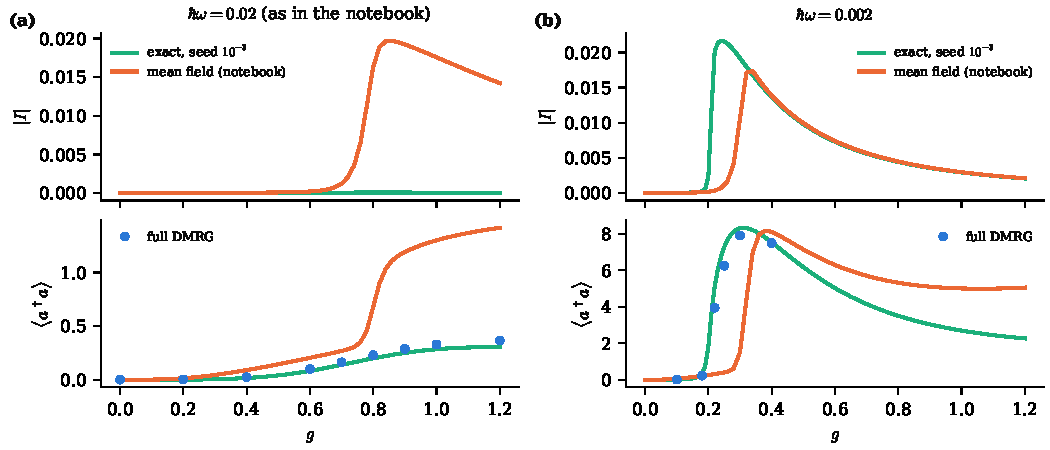
\includegraphics[width=\textwidth]{../figs/fig_notebook_omega.pdf}
  \caption{\label{fig:notebook_omega}%
  Model of the original notebook (Zeeman-polarized dot, $L=11$, $t=2$, $\Delta=0.6$):
  current (top) and photon number (bottom) versus $g$ for (a) $\hbar\omega=0.02$ and
  (b) $\hbar\omega=0.002$. Green: exact (adiabatic, seed $10^{-3}$); orange: mean field;
  circles: full DMRG (photon number; these older runs predate the two-start protocol).}
\end{figure*}

\paragraph*{Experimental scales and signatures.}
The two control parameters are
$\beta=2\pi L I_c/\Phi_0$ and $E_J/\hbar\omega$, related by
$\beta=2\pi(Z/R_Q)(E_J/\hbar\omega)$, with $E_J/h\simeq0.5\,{\rm GHz}\times I_c[{\rm nA}]$.
Three classes of $\pi$ elements span the phase diagram
[Fig.~\ref{fig:overview}(b)]:
(i) SFS junctions ($I_c\sim1$--$100\,\mu$A) reach $\beta>1$ with geometric
inductances of a few to a few hundred pH and $E_J/\hbar\omega\sim10^2$--$10^4$.
This is the classical limit, where the half-flux state is fully polarized,
consistent with the spontaneous currents observed in SFS
and $d$-wave $\pi$ loops~\cite{Tsuei2000,Ryazanov2001,Bauer2004}.
(ii) Quantum-dot $\pi$ junctions in the doublet regime
($I_c^\pi\sim0.1$--$10$\,nA) require $L\sim0.03$--$3\,\mu$H, i.e.\ superinductances
(Josephson-junction arrays, granular Al) as in fluxonium circuits~\cite{Manucharyan2009,Grunhaupt2019}; this is the $\pi$-qubit regime of Refs.~\cite{Ioffe1999,Yamashita2005,Feofanov2010}. These give
$E_J/\hbar\omega\sim1$--$3$, and the exact diagram is unambiguous there: for
$E_J/\hbar\omega\lesssim2.5$ no current-carrying phase exists at any coupling $g\le0.4$, even where
$\beta$ reaches $2.7$ (the $U=8\Delta$ line of Fig.~\ref{fig:phaseUG}). The ground state is the
cat state $(|{\circlearrowright}\rangle+|{\circlearrowleft}\rangle)/\sqrt2$ with
$\delta\sim\hbar\omega$, and the crossover appears as a dip in the
$|0\rangle\to|1\rangle$ frequency and a jump in the transition matrix element
$\langle0|\Phi|1\rangle$, accessible in two-tone spectroscopy. A mean-field description
predicts a persistent current of $0.6I_c$ in this regime; it is absent.
(iii) Multichannel or gate-tunable $\pi$ junctions with
$I_c\sim50$--$200$\,nA in a high-kinetic-inductance loop ($L\sim3$--$40$\,nH,
$\omega/2\pi\sim2$--$5$\,GHz) give $\beta\sim1$--$10$ and $E_J/\hbar\omega\sim10$--$30$.
This is the regime of the phase diagram (Figs.~\ref{fig:phaseUG},~\ref{fig:phaseslices}) and of
Figs.~\ref{fig:udot} and~\ref{fig:halfflux}, worked out above for $I_c=100$\,nA and a $5$\,GHz mode:
a well-defined current-carrying state of $\simeq0.9I_c$ at $\beta\simeq1.3$--$2$, whose residual tunnelling
$\delta/\hbar\omega\sim10^{-4}$--$10^{-8}$ remains a measurable macroscopic-quantum-tunnelling signature,
and a threshold that lies $10$--$20\%$ above the classical $\beta=1$ in $g$.
In the externally biased realization, the half-flux bias must be stable to
$|\delta\Phi|\ll\delta/2I^\star$, i.e.\ $\lesssim10^{-6}\Phi_0$ for the parameters above.
The interaction-driven realization has no such requirement.

Two signatures distinguish the microscopic $\pi$ loop from a classical $\pi$ loop with a fixed
Josephson energy. First, the $0$ phase is not inert: for $U<U_c(g)$ the mode is stiffened,
$\omega'/\omega=\sqrt{1+2g^2E''(0)/\hbar\omega}$ up to $9.4$ at $g=0.4$ here, and its ground state is a
squeezed vacuum whose photon number reproduces the DMRG value to $1\%$. A resonator frequency that
\emph{rises} with the coupling in the $0$ phase and softens towards the condensation in the $\pi$ phase
tells which side of $U_c$ the junction is on, independently of the current, and is directly
accessible in transmission. Second, the mode itself moves the $0$--$\pi$ boundary: a gate that tunes
$U/\Gamma$ across the window $0.85\Delta<U<0.94\Delta$ switches the parity of the junction at a
coupling-dependent point $U_c(g)$, $0.09\Delta$ below the zero-flux crossing at $g=0.4$. This parity
switch is a prediction of the microscopic treatment; the effective circuit model reproduces it only
with the exact singlet surface, and mean field, which replaces the Kramers doublet by a static
moment, places it at $0.82\Delta$ for every $g$.

\bibliography{refs}
\clearpage
% ==================================================================
%  Supplemental Material
% ==================================================================
\onecolumngrid
\begin{center}
{\large\bf Supplemental Material}
\end{center}
\setcounter{figure}{0}
\renewcommand{\thefigure}{S\arabic{figure}}
\renewcommand{\theHfigure}{S\arabic{figure}}
\setcounter{equation}{0}
\renewcommand{\theequation}{S\arabic{equation}}
\renewcommand{\theHequation}{S\arabic{equation}}
\twocolumngrid

\paragraph*{S1. Gauge covariance of the static phase and the circuit meaning of the one-bond vertex.}
For a static phase the position of the Peierls factor is a gauge choice: with the pairing transformed
covariantly, $\Delta_j\to\Delta e^{-2i\theta_j}$, a uniform vector potential along the ring gives the same
BdG spectrum as the full phase on the junction bond (prescription of Ref.~\cite{Dmytruk2021}; verified
to $10^{-10}$ for $\varphi=0$--$\pi/2$; a uniform
vector potential with a \emph{real} $\Delta$ is not equivalent). For the quantized flux the unitary
$W=\exp[-ig(a+a^\dagger)\sum_j\lambda_jn_j]$ that moves a fraction $\lambda_j$ of the phase onto bond $j$
does not commute with $\hbar\omega a^\dagger a$~\cite{DmytrukTrifSimon2016}: with $N=\sum_j\lambda_jn_j$
and $P=-i(a-a^\dagger)$, $W^\dagger a^\dagger aW=a^\dagger a+gNP+g^2N^2$, so that the two placements differ
by $\hbar\omega g(NP+gN^2)$, a coupling of the electron charge on the displaced sites to the charge of the
mode. In a lumped circuit this term is the capacitive coupling of the mode to the ring segment that carries
the vector potential; Eq.~(1) of the main text is the circuit in which the voltage of the mode drops across
the junction, the only high-impedance element of the loop. The neglected terms are of relative order
$\hbar\omega g^2/E_A$: $10^{-3}$ on the phase diagram, $10^{-2}$--$10^{-1}$ at the largest $\hbar\omega$ and $g$ of
Fig.~2, where the flux-driven switch is already fully developed at $\hbar\omega=0.01\Delta$.

\paragraph*{S2. Junction at $g=0$ and the $\pi'$ window.}
Figure~\ref{fig:junctions} characterizes the junction alone. DMRG in the even and odd parity sectors gives
the $0$--$\pi$ transition of the Anderson impurity between BCS
leads~\cite{Vecino2003,Karrasch2008,MengFlorensSimon2009,Zitko2015}. At $U=2\Delta$,
$E_2=+7.39\times10^{-3}\Delta$ with $|E_1|/E_2=2\%$ and $|E_4|/E_2<1\%$: a pure $\pi$ junction,
indistinguishable after normalization from a weak link biased by $\Phi_0/2$ [Fig.~\ref{fig:junctions}(a)].
$E_2$ decreases monotonically with $U$ ($\propto U^{-1.3}$ for $4\Delta\le U\le8\Delta$, approaching the
$1/U$ of cotunnelling through the singly occupied level). Three crossings of the two sectors are distinct
[Fig.~\ref{fig:junctions}(b)]: the zero-flux crossing $U_c^0=0.94\Delta$, the crossing of the global minima
$E_{\rm odd}(\pi/2)=E_{\rm even}(0)$ at $0.85\Delta$, and the crossing at half a flux quantum below it. The
window $0.85\Delta<U<0.94\Delta$ is the $\pi'$ phase~\cite{Vecino2003,Karrasch2008}: the singlet is the
ground state at zero flux, but the global minimum of $E(\varphi)$ belongs to the doublet at $\Phi_0/2$. The
singlet surface has a cusp at $\varphi=\pm\pi/2$, where two even-parity states cross, and is represented by
a spline through $25$ phases in the circuit model; the doublet surface is a smooth $\cos2\varphi$ with $2\%$
corrections. The strong junction used in the feasibility estimate ($t_J=t$, $\Gamma=2\Delta$) has
$U_c^0=5.55\Delta$ and, at $U=6\Delta$, $E_2=0.034\Delta$, $E_{\rm odd}-E_{\rm even}=-0.044\Delta$ at zero flux
and $|E_1|/E_2=1\%$ ($L=14$); its full-DMRG scan at $\hbar\omega=0.003t$ gives a condensate of $9.6$ photons
and $0.94I_c$ at $g\simeq0.12$, in agreement with the circuit model to $1\%$.

\begin{figure*}
  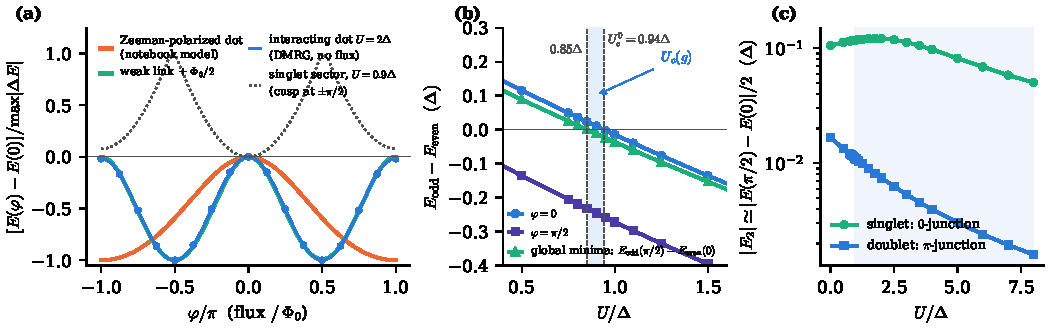
\includegraphics[width=\textwidth]{../figs/fig_junctions.pdf}
  \caption{\label{fig:junctions}%
  (a) Normalized $E(\varphi)$ of the loop for a Zeeman-polarized dot in a short ring (dominated by the
  $h/e$ harmonic), a weak link biased by $\Phi_0/2$ ($L=14$) and the interacting dot at $U=2\Delta$ without
  bias ($L=10$; symbols: DMRG; line: cosine fit); dotted: the singlet surface at $U=0.9\Delta$ with its cusp.
  (b) $E_{\rm odd}-E_{\rm even}$ at $\varphi=0$, at $\varphi=\pi/2$ and between the global minima
  (DMRG, $L=10$, $t_J=0.5\Delta$); shaded: the $\pi'$ window in which the boundary of the loop moves with $g$.
  (c) $|E_2|$ in the singlet and doublet sectors.}
\end{figure*}

\paragraph*{S3. DMRG protocol.}
The ring is stored in folded order next to the bosonic site, so that all ring bonds have range $\le2$
and the vertex $Dc^\dagger_{1\sigma}c_{0\sigma}$ is a three-site operator. Fermion parity and $S^z$ are
conserved. Benchmarks: at $g=0$ the energies of the non-interacting ring agree with exact BdG to
$10^{-14}$ at $\chi=1024$; for a four-site ring with a photon, DMRG reproduces exact diagonalization and the
sum rule $\langle I\rangle=(e/\hbar)(\hbar\omega/2g)\langle X\rangle$ to $10^{-7}$. On the phase diagram
$\chi=300$ (truncation error $<2\times10^{-8}$; $\chi=400$ changes the energies by $<4\times10^{-8}\Delta$ and
the current by $<0.3\%$ away from the crossover points) and $N_{\rm ph}=50$--$62$ (last Fock weight
$<10^{-7}$; $N_{\rm ph}=80$ changes the energy by $<10^{-9}\Delta$). The relevant criterion is not the energy:
the two current states are split only by $\delta$ and by the seed, $2I^\star\varphi_{\rm cl}\sim10^{-5}\Delta$,
and the local updates of DMRG drift towards the polarized state over tens of sweeps and can stop in an
under-polarized state whose energy is within $10^{-6}\Delta$ of the ground state. Every seeded point is
therefore started from two independent states, a warm start from the neighbouring point on the vacuum side
and a product state with the mode in a coherent state at the classical flux, converged first with seeds
$10^{-2}$ and $3\times10^{-3}$ and then relaxed at $10^{-3}$; the lower energy is kept when the two differ by
more than $3\times10^{-7}\Delta$, otherwise the pair is reported as a bracket ($47$ of $427$ points, all inside
the crossover windows); a state is accepted only if it satisfies the sum rule to $10^{-3}I_c$ (median
$10^{-4}I_c$); and the current above threshold must be independent of the seed (seed $10^{-4}$: unchanged to
$0.4\%$ above threshold, reduced by the factor $0.09$ below) [Fig.~\ref{fig:phaseconv}]. An earlier version
of these scans evaluated the observables after a warm start with the displacement operator of the previous
$g$; the sum rule exposed this error. For the seed-free runs (cat state, flux-driven switch) the symmetric
state is the ground state in each sector and no such care is needed; on the grid of Fig.~2 ($\hbar\omega=0.01$--$3\Delta$, $\chi=200$,
$N_{\rm ph}=16$--$48$) the truncation error is $<4\times10^{-7}$ and the last Fock weight $<4\times10^{-8}$, and the
boundary $U_c$ is obtained by linear interpolation of $E_{\rm odd}-E_{\rm even}$ between $U$ nodes $0.1$--$0.2\Delta$ apart
(adding nodes $0.05$--$0.1\Delta$ apart moves $U_c$ by $<10^{-3}\Delta$; $\chi=300$ changes the energies by $<5\times10^{-6}\Delta$ and the
difference by $<4\times10^{-6}\Delta$, $N_{\rm ph}=40$--$80$ by $<10^{-7}\Delta$); the photon--electron entanglement
entropy is computed from the photon reduced density matrix. The circuit model is diagonalized in a Fock
space of $200$ states (DVR in the eigenbasis of $X$); for the tunnel splitting below $10^{-6}\hbar\omega$ the
two flux-parity blocks are diagonalized separately, which gives $\delta$ as a difference of two
independently converged energies ($6.46\times10^{-9}\hbar\omega$ against $6.51\times10^{-9}$ from the full matrix
at $\beta=3$, $E_J/\hbar\omega=10$; at $E_J/\hbar\omega=40$ both are at the double-precision floor
$\sim10^{-9}\hbar\omega$ for $\beta\ge1.25$).

\begin{figure*}
  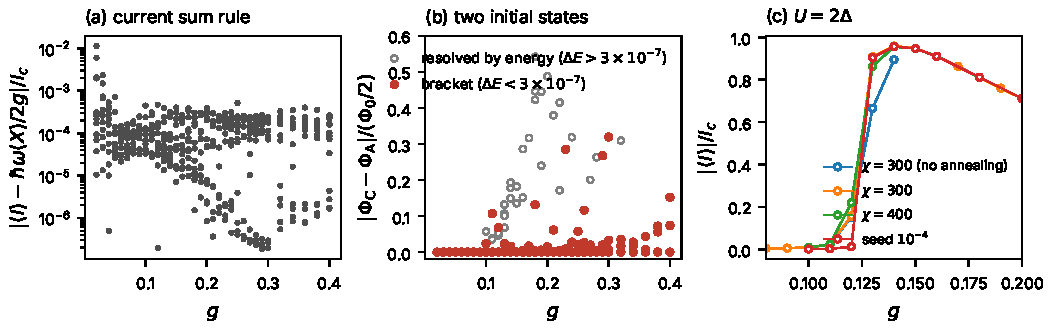
\includegraphics[width=\textwidth]{../figs/fig_phase_convergence.pdf}
  \caption{\label{fig:phaseconv}%
  Convergence of the full DMRG on the phase diagram. (a) Violation of the sum rule over the grid.
  (b) Difference between the fluxes of the two initial states (vacuum side A, polarized side C) in units of
  $\Phi_0/2$: open symbols resolved by the energy, filled reported as brackets. (c) $U=2\Delta$ near threshold:
  $\chi=300$ without and with the annealed start, $\chi=400$, and seed $10^{-4}$.}
\end{figure*}


\begin{figure*}
  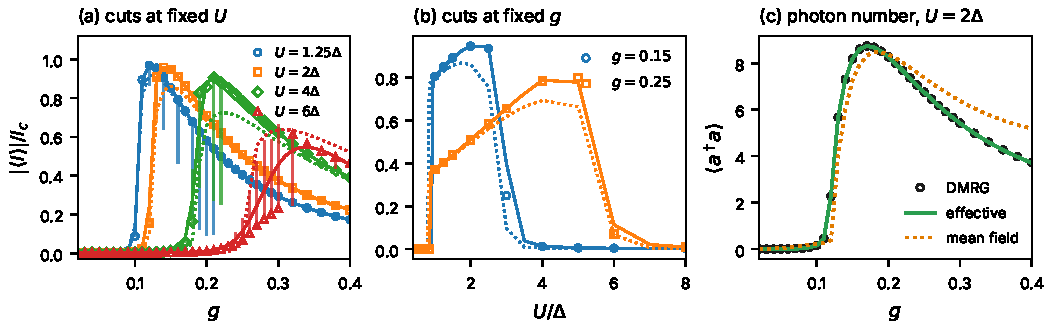
\includegraphics[width=\textwidth]{../figs/fig_phase_slices.pdf}
  \caption{\label{fig:phaseslices}%
  Cuts through Fig.~2 of the main text. (a) Current versus $g$ at $U/\Delta=1.25,2,4,6$ and (b) versus
  $U$ at $g=0.15,0.25$: full DMRG (symbols; bars: bracket between the two initial states), circuit model
  (solid), mean field (dotted). (c) Photon number at $U=2\Delta$.}
\end{figure*}

\paragraph*{S4. Half-flux-biased weak link.}
For an ordinary weak link ($L=14$, $t_J=0.5$, $E_2=-0.056\Delta$, $E_1=-5.4\times10^{-4}\Delta$, Andreev gap
$0.77\Delta$) biased by $\Phi_0/2$, Fig.~\ref{fig:halfflux} shows the full DMRG at $E_J/\hbar\omega=10$ versus
$\beta$. The current rises at $\beta\simeq1.1$, saturates at $0.96I_c$ for $\beta\approx1.7$ and then
decreases as the flux approaches $\Phi_0/2$. DMRG and the circuit model agree to $2\times10^{-3}\hbar\omega$
in energy, $2\%$ of $I_c$ in current and $1.3\%$ in $E_1-E_0$. The product state is $0.2$--$0.4\hbar\omega$
too high in energy and overestimates the current threefold near threshold ($0.71I_c$ against $0.22I_c$ at
$\beta=1.13$). The direction of the current is selected by the residual $h/e$ harmonic, which tilts the double
well by $2|E_1|\sin\varphi^\star\approx0.2\hbar\omega$ and sets $E_1-E_0$ for $\beta>1.2$; without it
$\delta/\hbar\omega$ would fall below $10^{-6}$ at $\beta=2$. The flux distribution evolves from a Gaussian
at zero to a single displaced peak.

\begin{figure*}
  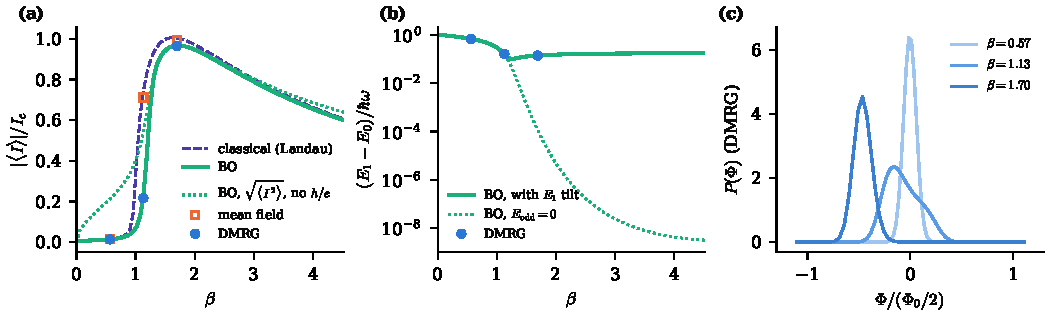
\includegraphics[width=\textwidth]{../figs/fig_weaklink_halfflux.pdf}
  \caption{\label{fig:halfflux}%
  Weak-link loop ($L=14$) biased by $\Phi_0/2$, $E_J/\hbar\omega=10$. (a) Persistent current versus $\beta$:
  DMRG (circles), MF (squares), circuit model with (solid) and without (dotted) the odd harmonics, classical
  Landau theory (dashed). (b) Splitting of the two lowest levels. (c) Flux distribution of the DMRG ground state.}
\end{figure*}

\paragraph*{S5. Product state at $E_J\simeq\hbar\omega$.}
The product-state mean field is the method of Refs.~\cite{Varrica2026,Andolina2020} and of our own earlier
treatment of this circuit: Hartree--Fock BdG electrons with the junction bond renormalized by
$\alpha=\langle D\rangle$, times the ground state of $\hbar\omega a^\dagger a-(\eta D+{\rm h.c.})$ with
$\eta=t_Je^{i\varphi}\langle c^\dagger_1c_0\rangle$, iterated to self-consistency. For a Zeeman-polarized dot
in a short BCS ring ($t=2$, $\Delta=0.6$, $L=11$, $\epsilon_{d\uparrow}=-0.3$, $\epsilon_{d\downarrow}=3.7$,
$t_J=0.5$, $\hbar\omega=0.02$; energies in units of $t$) it predicts a current-carrying phase for
$g\gtrsim0.75$ with $|\langle I\rangle|\approx0.02$ and $\langle a^\dagger a\rangle\simeq1$--$1.4$. DMRG shows
that this phase is an artefact [Fig.~\ref{fig:notebook}]: the exact energy lies below the MF energy by up to
$1.8\hbar\omega$, the gap to the first excited state stays at $0.33\hbar\omega$, the photon number saturates at
$0.36$ and the response to the seed is linear, $\langle I\rangle\approx7\times10^{-5}$. Two effects are
responsible. (i) The product state is not gauge covariant: with the full Peierls phase on one bond it
renormalizes that bond by $|\langle D\rangle|<1$ and loses phase-\emph{independent} kinetic energy, which the
exact state recovers by following the flux. (ii) $E_J\simeq\hbar\omega$: the Landau energy develops a double
well for $g>0.58$, but its depth is below the zero-point energy and $P(X)$ stays unimodal. In this ring
$L\lesssim\xi$ and $E(\varphi)$ is dominated by the $h/e$ harmonic ($E_1=2.1\times10^{-2}\gg E_2=2\times10^{-3}$),
which is why all other results use $L\gg\xi$. At $\hbar\omega=0.002$ the same model does order, at
$g_c\simeq0.21$, while mean field gives $0.30$.

\begin{figure}
  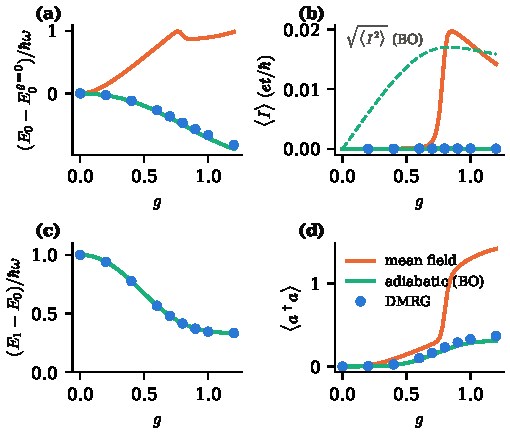
\includegraphics[width=\columnwidth]{../figs/fig_notebook_model.pdf}
  \caption{\label{fig:notebook}%
  Short ring with a Zeeman-polarized dot ($\hbar\omega=0.02$, seed $10^{-3}$): mean field (orange), circuit
  model (green) and DMRG (symbols). (a) Energy, (b) current (dashed: rms current of the circuit-model ground
  state), (c) gap to the first excited state, (d) photon number.}
\end{figure}

\paragraph*{S6. Physical units.}
With $E_J/h=0.5\,{\rm GHz}\times I_c[{\rm nA}]$ and $\beta=2\pi(Z/R_Q)(E_J/\hbar\omega)$:

\begin{center}\scriptsize
\begin{tabular}{lccccc}
\hline
junction, material & $E_J/h$ & $I_c$ & $E_J/10h$ & $E_J/10k_B$ & $L_{\beta=1}$ \\
\hline
$2\Delta$, $\Delta/2$, Al & 0.32 GHz & 0.65 nA & 32 MHz & 1.5 mK & 510 nH \\
$2\Delta$, $\Delta/2$, NbTiN & 2.1 GHz & 4.3 nA & 210 MHz & 10 mK & 76 nH \\
$6\Delta$, $2\Delta$, Al & 1.5 GHz & 3.0 nA & 150 MHz & 7 mK & 110 nH \\
$6\Delta$, $2\Delta$, NbTiN & 9.9 GHz & 20 nA & 0.99 GHz & 47 mK & 17 nH \\
$6\Delta$, $2\Delta$, Nb & 11.5 GHz & 23 nA & 1.15 GHz & 55 mK & 14 nH \\
\hline
\end{tabular}
\end{center}
(first column: $U$, $\Gamma$, superconductor; $L_{\beta=1}=\Phi_0/2\pi I_c$).
The flux-driven switch needs none of this: $\hbar\omega=0.1\Delta$ is $4.4$\,GHz in Al and $g=0.5$ is
$Z=2.0\,{\rm k}\Omega$.

\end{document}
